%
% Exemplo LaTeX de artigo UNISINOS
%
% Elaborado com base nas orientações dadas no documento
% ``GUIA PARA ELABORAÇÃO DE TRABALHOS ACADÊMICOS''
% disponível no site da biblioteca da Unisinos.
% http://www.unisinos.br/biblioteca
%
% Os elementos textuais abaixo são apresentados na ordem em que devem
% aparecer no documento.  Repare que nem todos são obrigatórios - isso
% é devidamente indicado em cada caso.
%
% Comentários abaixo colocados entre aspas (`` '') foram
% extraídos diretamente do documento da biblioteca.
%
% Este documento é de domínio público.
%

%=======================================================================
% Declarações iniciais identificando a classe de documento e
% selecionando alguns pacotes adicionais.
%
% As opções disponíveis (separe-as com vírgulas, sem espaço) são:
% - twoside: Formata o documento para impressão frente-e-verso
%   (o default é somente-frente)
% - english,brazilian,french,german,etc.: idiomas usados no documento.
%   Deve ser colocado por último o idioma principal.
%=======================================================================
\documentclass[twoside,english,brazilian]{UNISINOSartigo}
\usepackage[utf8]{inputenc} % charset do texto (utf8, latin1, etc.)
\usepackage[T1]{fontenc} % encoding da fonte (afeta a sep. de sílabas)
\usepackage{graphicx} % comandos para gráficos e inclusão de figuras
\usepackage{bibentry} % para inserir refs. bib. no meio do texto
\usepackage{enumitem}
\usepackage[section]{placeins}
\usepackage{float}
\usepackage{tabularx}
\usepackage{array}
\usepackage{caption}
\usepackage{listings}
\usepackage{ltxtable}
\usepackage{pdfpages}
\usepackage{setspace}
\usepackage{breakcites}

%\usepackage{url}
%\usepackage{breakurl}
%\usepackage[breaklinks]{hyperref}
%=======================================================================

\unisinosbst
%\usepackage{xcolor}
\usepackage[dvipsnames]{xcolor}
%\usepackage[alf]{abntcite}
%Ajustando a source para figuras
\newcolumntype{L}{>{\centering\arraybackslash}m{8cm}}
\newcommand{\source}[1]{\caption*{Fonte: {#1}} }
\long\def\/*#1*/{}

\definecolor{persiangreen}{rgb}{0.0, 0.65, 0.58}

%Ajustando espaços em branco das figuras
\setlength{\abovecaptionskip}{2.0pt}
\setlength{\belowcaptionskip}{-6pt}


%=======================================================================
% Capa
%=======================================================================
\newcounter{mypagecount}% create a new counter
\setcounter{mypagecount}{0}% set it to something just in case
\newenvironment{interlude}{% create a new environment for the unnumbered section(s)
  \clearpage
  \setcounter{mypagecount}{\value{page}}% use the new counter we created to hold the page count at the start of the unnumbered section
  \thispagestyle{empty}% we want this page to be empty (adjust to use a modified page style)
  \pagestyle{empty}% use the same style for subsequent pages in the unnumbered section
  }{%
  \clearpage
  \setcounter{page}{\value{mypagecount}}% restore the incremented value to the official tally of pages so the page numbering continues correctly
  }
\usepackage{lipsum}

%=======================================================================
% Início do documento.
%=======================================================================
\begin{document}
\begin{interlude}

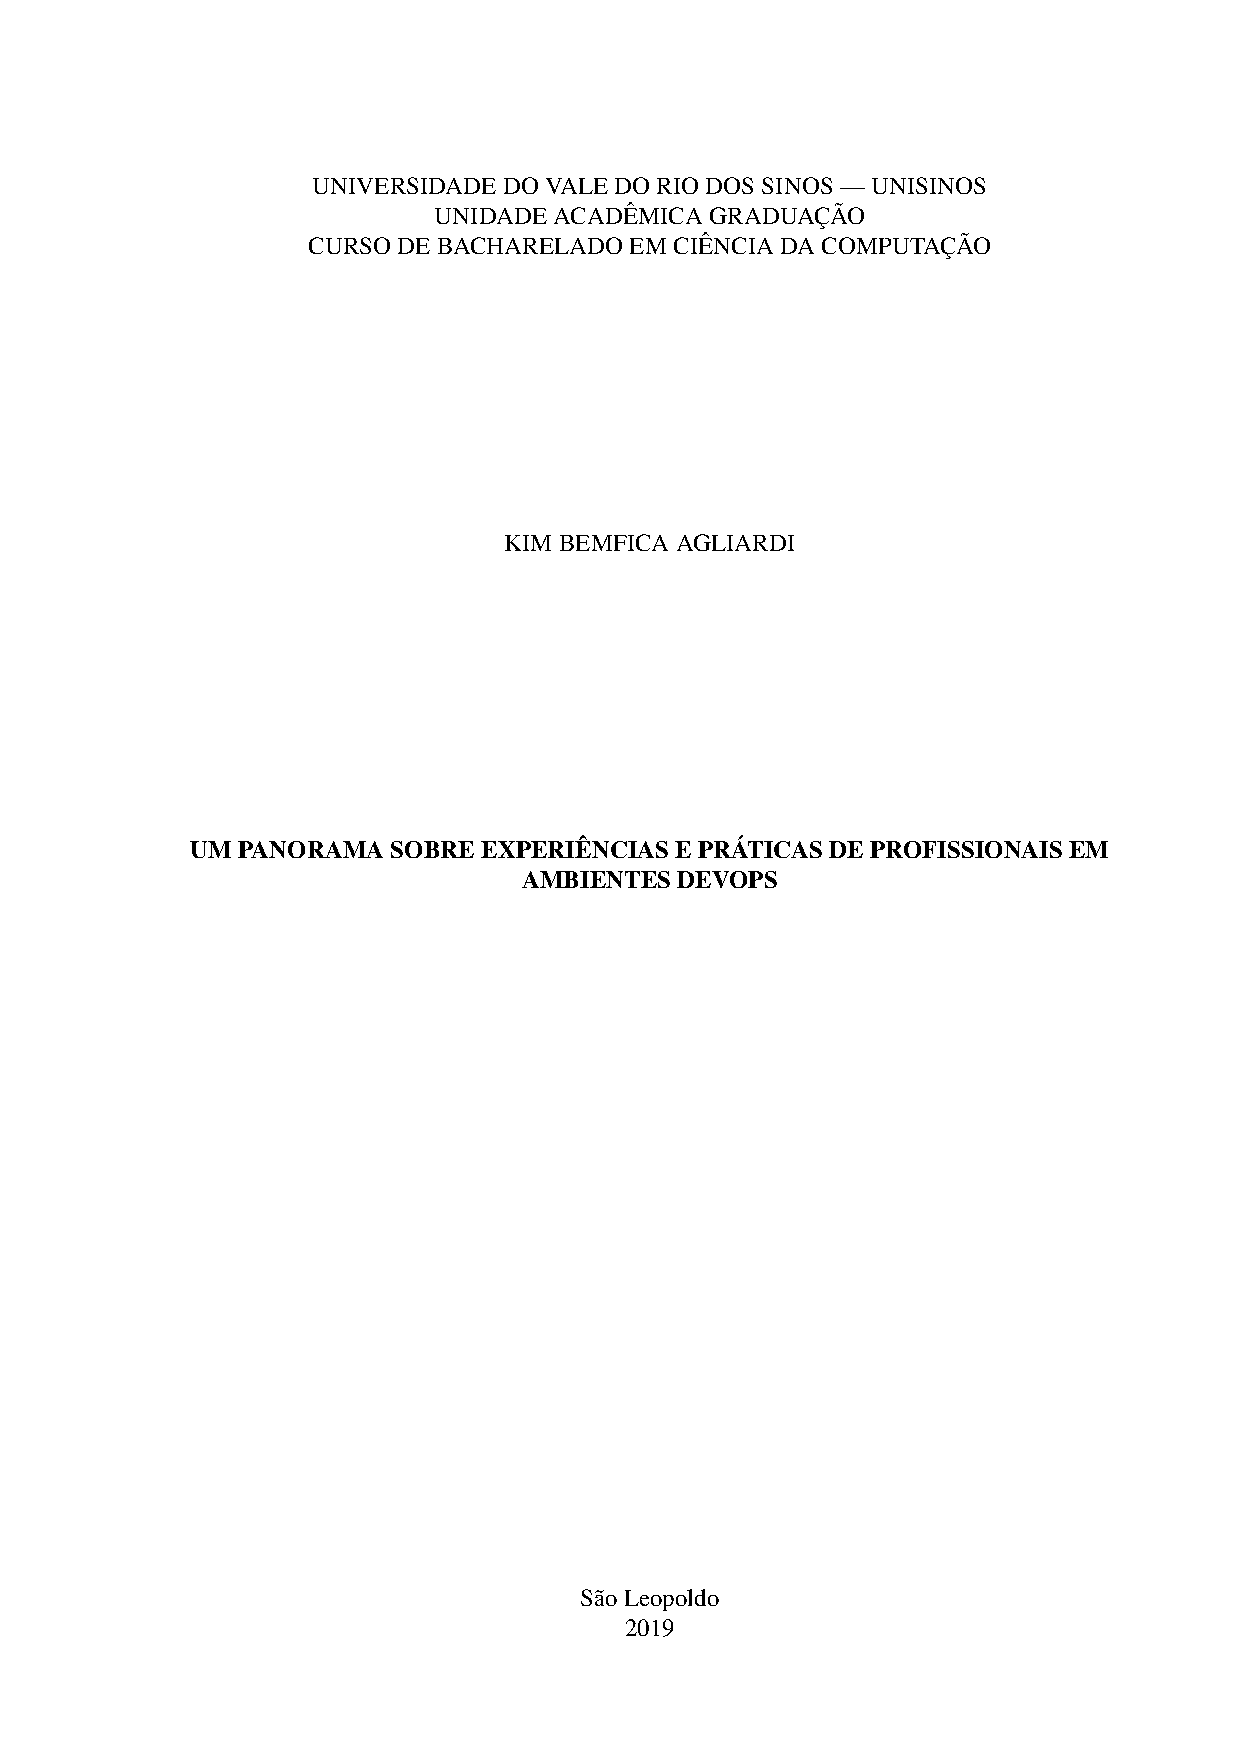
\includepdf[pages={1,3}]{capa.pdf}
\end{interlude}
% Diferentemente do normal, os comandos a seguir devem vir aqui mesmo,
% e não antes do \begin{document} onde seria o lugar deles. 
\titulo{Um panorama sobre experiências e práticas de profissionais em ambientes DevOps.}
\autor{Kim Bemfica Agliardi\footnote{Aluno do curso de Ciência da Computação.  Email: kim.agliardi@gmail.com}}
\autor{Christopher da Rosa Pohlmann \footnote{Orientador, professor da Unisinos, Mestre em Engenharia de Produção e Sistemas pela Universidade do Vale do Rio dos Sinos(2009)  Email: chrisp@unisinos.br}}

%=======================================================================
% Resumo em Português.
%
% A recomendação é para 150 a 250 palavras.
%=======================================================================
\begin{abstract}
Ao longo dos últimos anos a cultura de DevOps tem ganhado força no mercado de tecnologia da informação (TI). O seu principal objetivo é o alinhamento entre as equipes de desenvolvimento e operação, para que juntos os times realizem entregas mais rápidas e de qualidade, por meio de ferramentas e responsabilidades previamente definidas. Trata-se de uma cultura de colaboração entre as equipes. Este estudo tem como objetivo realizar um panorama sobre os profissionais que estão trabalhando em organizações que praticam a cultura DevOps, entendendo qual é o seu nível de experiência no mercado de TI e quais práticas de DevOps estão em uso por estes profissionais, bem como mapear dificuldades encontradas por estes profissionais ao longo de implantações de ferramentas de automação, também pretendemos mapear quais recursos são utilizados na busca de novos conhecimentos por estes profissionais.

\palavraschave{DevOps\@. Infraestrutura como código\@. Metódos Ágeis \@. Entrega Contínua \@. Integração Contínua. \@ }
\end{abstract}

%=======================================================================
% Introdução
%=======================================================================
\section{Introdução}

%Ao longo dos últimos anos foi possível observar um crescimento na importância das áreas de TI, fato que até então, não era verdade. 
\citetexto{Beal2009} lembra que ``por muito tempo a Tecnologia da Informação (TI) foi considerada um ``centro de custo''  e que em princípio não gerava qualquer retorno para o negócio'', dando ênfase aos altos valores de investimento em equipamentos e o pouco uso que se fazia destes.  Atualmente, as organizações vêm enfrentando um ambiente extremamente competitivo, inseridas em uma sociedade profundamente afetada pelos novos paradigmas introduzidos pela chamada sociedade da informação. A nova realidade provoca a reorganização intensa da sociedade, gerando modificações nas organizações. Neste contexto, as áreas de sistemas de informação tem se tornado cada vez mais críticas, dado o constante clima de mudança.  \cite[p. 15]{AudyFreitag08}.

Com toda essa competitividade existente no mercado, mudanças de software tornaram-se comuns para as empresas, que até então, não estavam habituadas a realizar mudanças tão constantes em suas aplicações. O aumento no ritmo de entrega de software evidenciou a disparidade existente entre as equipes de desenvolvimento e operações de TI existentes nas organizações. Enquanto equipes de desenvolvimento, de um modo geral, possuem metodologias, frameworks e ferramentas bem estruturadas, que automatizam etapas de desenvolvimento de software e tratam do ciclo de vida de uma aplicação, equipes de operações de TI ainda  não estão tão bem estruturadas, realizando diversas tarefas de maneira manual e com uma baixa padronização. 
Confome observado por \citetexto{Debois2008} infraestrutura também podem adotar algumas das práticas já existentes e utilizadas por equipes de desenvolvimento, e a partir dos questionamentos levantados em seu artigo ``\textit{Agile and Operations Infrastructure: How Infra-gile Are You}?'', um grupo de discussão denominado ``\textit{Agile-Sysadmin}''  foi criado. Neste grupo passou-se debater a ideia de adoção de práticas ágeis e de automação para equipes de infraestrutura. Essa iniciativa é considerada por muitos, o nascimento da cultura DevOps. O DevOps também e visto como uma evolução natural dos métodos ágeis, que foi estendido e passou à atender também áreas de operação. 

É importante salientar que diferente do movimento ágil ou Information Technology Infrastructure Library(ITIL), DevOps não possui uma ``metodologia'' para implementação, ou até mesmo, um manifesto que direcione seu processo de adoção, o que acaba tornando esta tarefa um pouco mais complexa. Dado este contexto, diversos estudos buscam uma definição sobre o que é DevOps, quais são seus processos e práticas, formas de implementar a cultura e quais são as características (habilidades e experiências) que as companhias buscam nos profissionais que vão compor estas equipes.

%\subsection{Motivação}
DevOps é um assunto abrangente, e por muitos é considerado uma cultura e não apenas uma coleção de práticas de automação, pois além de se debater o lado técnico, existe uma grande dicussão sobre o lado comportamental/cultural. Por ser um assunto recente, encontram-se muitos estudos propondo o que é DevOps e quais são suas práticas relacionadas. Observa-se também alguns poucos artigos acadêmicos relacionados aos profissionais e qual o entendimento destes sobre a importância do tema DevOps em sua rotina de trabalho, a maior parte dos artigos relacionados a essa temática são encontrados na indústria. Diante deste contexto surge a seguinte pergunta de pesquisa: Quais são as características dos profissionais que estão inseridos em ambientes que promovem a cultura DevOps?

%\subsection{Objetivo Geral}
Desta forma, este estudo tem como objetivo geral analisar as características dos profissionais que estão inseridos em ambientes que promovem a cultura DevOps. Esse objetivo desdobra-se nos seguintes objetivos específicos: (a) apresentar dados sócio-demográficos dos grupos DevOps BR, DevOps Porto Alegre e Docker Porto Alegre. (b) analisar o nível de colaboração entre as equipes de desenvolvimento e operação; (c) analisar o nível de maturidade sobre práticas DevOps; (d) analisar o uso de ferramentas DevOps; e, (e) analisar a percepção sobre a adoção da cultura DevOps, considerando atividades \textit{core} de DevOps/Release engineers, as fontes de informação sobre DevOps e principais benefícios e dificuldades.

%Nesta pesquisa essas características seguem organizadas em (a) dados sócio-demográficos, (b) nível de maturidade das práticas DevOps, (c) ferramentas e atividades, (d) fontes de informação, e (e) dados qualitativos sobre dificuldades e ganhos na adoção do DevOps.

%, entendendo quais são suas habilidades técnicas, grupos de ferramentas relevantes para a automação de processos, experiências e dificuldades encontradas por estes profissionais para sustentar as práticas de automação que são aplicadas neste novo paradigma de trabalho.

%\subsection{Objetivo específicos}

%referida análise desdobra-se no seguintes objetivos específicos:

% begin{enumerate}[label=\alph*)]
% \item Identificar experiências prévias destes profissionais no mercado de TI;
%    \item Identificar quais práticas relacionadas a DevOps estão em uso por estes profissionais, bem como em qual estágio de maturidade se encontram;
%    \item Analisar como estes profissionais estão se preparando em termos de estudo para este novo paradigma, bem como quais são suas fontes de informação sobre novas ferramentas e práticas;
%    \item Analisar a opinião destes profissionais sobre quais são as dificuldades e ganhos na adoção deste novo paradigma.
%\end{enumerate}
%*/

%\subsection{Metodologia}
%Esta pesquisa foi do tipo descritivo, de forma que os procedimentos foram classificados como descritivos.
Neste trabalho busca-se analisar quais são as características dos profissionais inseridos em companhias que estão adotando ou já adotaram as práticas da cultura DevOps. Para tanto, foi necessário realizar uma revisão bibliográfica para compreender quais são os pontos-chave desta cultura (ferramentas, frameworks e atividades consideradas \textit{core} para este novo papel). Baseado nos achados levantados durante esta revisão, elaborou-se um questionário com 27 questões, relacionadas a DevOps e experiências destes profissionais. 

%\subsection{Estrutura do trabalho}
O presente trabalho divide-se em cinco capítulos, dos quais o \textbf{primeiro capítulo} apresenta os objetivos, o método utilizado e a justificativa para o desenvolvimento do TCC. O \textbf{segundo capítulo} apresenta o referencial teórico, conceituando em linhas gerais o que é DevOps, quais são as características que esta cultura apresenta e uma breve descrição sobre as práticas utilizadas pelos profissionais. O \textbf{terceiro capítulo} apresenta-se as etapas de pesquisa. No \textbf{quarto capítulo} detalham-se os resultados do Survey e por fim, no \textbf{quinto capítulo} seguem as conclusões.
%=======================================================================
% Referencial Teórico
%=======================================================================
\section{REFERENCIAL TEÓRICO}

Ao longo desta seção, apresentam-se os principais conceitos sobre DevOps, como seus princípios, métodos e modelos, bem como as motivações que impulsionaram este movimento.

\subsection{A relação entre Desenvolvimento  e Operações/Infraestrutura}
Com a pressão constante para entrega de valor por meio de software aos clientes, não é incomum que áreas de desenvolvimento e operações entrem em conflito. Enquanto desenvolvedores buscam pôr em produção o mais brevemente possível novas funcionalidades/sistemas, equipes de operação preocupam-se com a estabilidade, o que significa não realizar alterações em sistemas de produção frequentemente.
Segundo \citetexto{HUTTERMANN12}, esses conflitos geram barreiras culturais e organizacionais, que ocasionam as seguintes situações:
Como o foco das equipes é diferente, a tensão entre as equipes aumenta e cada uma defende seus interesses individuais, sem pensar no todo; A lacuna destes processo resulta em diferentes abordagens entre Dev/Ops sobre como gerenciar mudanças, colocá-las em produção e mantê-las funcionando; A origem dessa lacuna começa pelas próprias ferramentas utilizadas pelas equipes, que geralmente são diferentes.

Existe um termo na indústria que descreve esse tipo de comportamento como ``O muro da confusão'', que é causado justamente pela combinação de diferentes motivações (cada equipe defende o seu ponto), processos mal formulados e diferentes ferramentas de trabalho. Como cada equipe acredita estar fazendo o correto pelo negócio, as decisões ocorrem de maneira isolada e este ``jogo de responsabilidades'' ocorre.

\begin{figure}[h!]
    \centering
        \caption{Muro da confusão}
    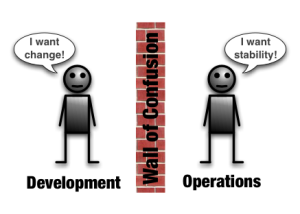
\includegraphics[scale=.6]{imagens/WallOfConfusion.png}
    \source{\citetexto{DEV2PS}}
    \label{fig:Muro da confusão}
    \end{figure}

É interessante observar que ao longo do tempo o processo de desenvolvimento de software sofreu diversos aprimoramentos, passando por modelos como o cascata (\textit{waterfall}) até chegar no padrão que é visto hoje, que é baseado em metodologias ágeis. Já áreas de operações geralmente baseiam-se em métodos como ITIL, que possui processos processos claros e bem definidos para cada etapa de vida de um serviço. Essa diferença processual segue o mesmo descompasso que é visto no ferramental utilizado pelas equipes, enquanto métodos ágeis visam a entrega de pequenas partes de um sistema de maneira constante, gerando um grande número de alterações em um breve período de tempo por meio de suas \textit{sprints}, o ITIL, por exemplo, com o processo de gerenciamento de mudanças, prevê um modelo formal com reuniões e discussões entre às equipes antes da realização de alguma alteração. 

\subsection{Métodos ágeis e DevOps}
O movimento ágil começou com a escrita do \textbf{Manifesto Ágil} por \citetexto{beck2001agile}, e o nome ``\textit{Agile}'' foi o nome dado ao conjunto de métodos de desenvolvimento de software que haviam sido desenhados para serem mais leves e flexíveis do que modelos como o cascata.
O que diz o manifesto ágil:  \newline

\begin{quote}
Estamos descobrindo maneiras melhores de desenvolver 
software, fazendo-o nós mesmos e ajudando outros a 
fazerem o mesmo. Através deste trabalho, passamos a valorizar: \textbf{Indivíduos e interações} mais que processos e ferramentas; \textbf{Software em funcionamento} mais que documentação abrangente; \textbf{Colaboração com o cliente} mais que negociação de contratos; \textbf{Responder a mudanças} mais que seguir um plano
Ou seja, mesmo havendo valor nos itens à direita, os itens mais à esquerda são mais valorizados.
\end{quote}

É importante perceber que o principal objetivo do movimento ágil é enfatizar a colaboração, flexibilidade e como resultado final, diminuir o tempo de entrega de \textit{software}, diminuir o valor gasto e fornecer um \textit{software} de qualidade. Porém, os métodos ágeis não definem práticas para a disponibilização do \textit{software}, o que acaba gerando uma lacuna entre as equipes de desenvolvimento e operação. Apesar do aumento de performance gerado pela adoção de práticas ágeis, existe a demora da fase de implantação do \textit{software}, que em muitos casos, é causado pelo medo de ``quebra'' da aplicação à cada nova funcionalidade ou correção integrada a solução, por parte da equipe de operações, que tem como foco a estabilidade da aplicação.
O modelo ágil é próximo ao DevOps tanto no sentido cultural, isto é, o foco está nos indivíduos e na colaboração, quanto na redução de tempo de disponibilização de \textit{software}. As práticas de integração contínua, entrega contínua, testes contínuos e  infraestrutura como código, seguem justamente a ideia de não aguardar um ciclo inteiro para integrar, testar e disponibilizar, mas sim, integrar as funcionalidades assim que possível.

%\subsection{ITIL}
%A Information Technology Infrastructure Library (ITIL), é um conjunto de práticas definidas para o gerenciamento de serviços de TI. É uma publicação que contém 5 volumes que descrevem: Processos, procedimentos, tarefas e checklists e é utilizada por organizações para demonstrar conformidade e  medidas para melhoria de serviços \cite{Davis}. \newline
%Sua primeira versão foi publicada no final dos anos 80, e o número de livros e práticas cresceu com o passar dos anos, sua última publicação (ITIL V3) foi realizada no ano de 2011, e esta versão contém livros sobre: Estratégias de serviço, Design de serviço, Transição de serviço, Operação de serviço e Melhoria continuada. 
%Conforme observado por \citetexto{Borangiu2016}, métodos ágeis e ITIL possuem diferenças tanto conceituais como estruturais. Métodos ágeis são vistos como leves e flexíveis, enquanto ITIL é considerado burocrático e processual. Apesar de ambos possuírem o mesmo objetivo que é prover a entrega de valor ao negócio, no entanto, a maneira como isso é realizado é extremamente diferente para cada um destes frameworks. Enquanto métodos ágeis visam entregar rapidamente o que o cliente deseja, ITIL visa entregar serviços de TI estáveis, respeitando um conjunto de níveis de serviço e qualidade previamente acordados. O manifesto ágil favorece as interações informais entre os participantes do projeto, em oposição a um alto formalismo, que é defendido pelo ITIL.
%Dado esse contexto, é interessante observar que este é mais um ponto de dissidência presente entre as equipes de desenvolvimento e operações. Enquanto uma visa "fornecer valor" por meio da entrega rápida de funcionalidades (Dev) a outra busca um alto nível de estabilidade e satisfação do cliente (Ops), garantindo boas avaliações de nível de serviço e qualidade.



\subsection{DevOps}
%Nesta subseção aborda-se a origem do termo DevOps, suas principais características e práticas.

%\subsubsection{A origem da cultura "DevOps"}
A ideia sobre DevOps surgiu a partir de \citetexto{Debois2008} em seu artigo denominado ``\textit{Agile and Operations Infrastructure: How Infra-gile Are You?}''. A sua motivação para realização de sua pesquisa foi uma série de frustrações que ocorreram por conta de conflitos entre desenvolvedores e administradores de sistemas, ao longo de uma migração de um datacenter do governo Belga.  No ano de 2008 durante conferência AGILE '08 sobre práticas ágeis, realizada em Toronto, Patrick Debois e Andrew Shafer apresentaram o trabalho construído e também criaram um grupo de discussão denominado \textit{agile-sysadmin}, que inicialmente foi disseminado na Europa para discutir a adoção de metodologias ágeis na infraestrutura e entender como equipes de operação poderiam trabalhar no modelo ágil, acompanhando a equipe de desenvolvimento.

Tal iniciativa desencadeou uma série de estudos, conferências e iniciativas sobre o assunto, que engajou a comunidade à torná-lo popular. 
Um outro marco importante para o DevOps foi a conferência \textit{Velocity} da O'Really, realizada em 2009, onde foi apresentado o trabalho \textit{10+ Deploys per day: Dev and Ops Cooperation at Flickr}, por John Allspaw e Paul Hammond. Este trabalho foi um estudo de caso sobre a capacidade de implantação de mudanças no Flickr após pôr em prática a colaboração entre as equipes, priorizando a entrega de software de qualidade de maneira rápida e eficiente.
Esse estudo foi um marco para alavancar o movimento e nesta mesma conferência, surgiu a ideia de realizar o evento DevOpsDays\footnote{\url{https://devopsdays.org/}}, que é realizados em diversos países com grupos locais que tem como objetivo disseminar a cultura DevOps.

\subsubsection{O que é DevOps ?}

\textbf{DevOps} é um termo que se tornou uma \textit{buzzword} no mercado de TI e  por não ser prescritivo, muitas empresas tem apresentado a definição que lhes parece correta, bem como alguns profissionais que se intitulam ``DevOps'', um fenômeno que pode ser ilustrado pela Figura \ref{fig:elefante DevOps}.

\begin{figure}[h!]
    \centering
        \caption{O elefante DevOps}
    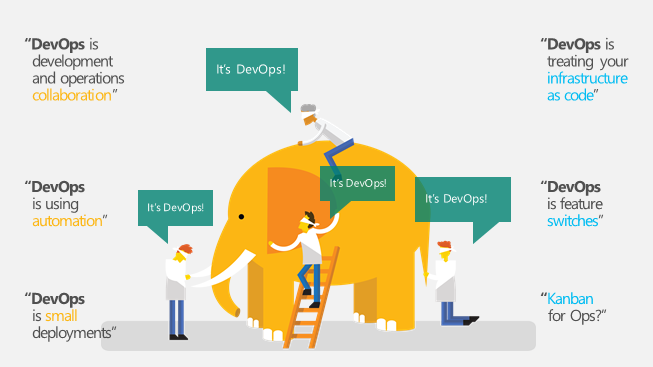
\includegraphics[scale=.6]{imagens/devops_elephant.png}
    \source{\citetexto{Microsoft2015}}
    \label{fig:elefante DevOps}
\end{figure}

Diferente das metodologias ágeis que possuem um manifesto ou ITIL que possui uma descrição sobre seus processos, não existe uma descrição exata sobre como ``ser DevOps'', pois ela é uma cultura definida por ideias e não por uma definição rigorosa. Segundo \citetexto{Davis} está em constante evolução, ou seja, processos e ideias tem sido discutidos ao longo dos últimos anos e pelo que se observa na comunidade, a tendência é de que permaneça assim ao longo dos próximos anos. 

A definição proposta por \citetexto{Jabbari2016} é de que DevOps é uma metodologia de desenvolvimento que busca eliminar os \textit{gap's} existentes entre Desenvolvimento e Operações. Também pode ser dito como um paradigma, método ou conjunto de princípios e práticas que possibilitam uma melhor comunicação e colaboração, resultando em um trabalho em equipe eficiente entre as equipes de desenvolvimento e operações.
Um acrônimo que é frequentemente citado nos grupos sobre DevOps é o CALMS, que significa \textbf{C}ulture, \textbf{A}utomation, \textbf{L}ean, \textbf{M}easurement e \textbf{S}haring. Esse acrônimo é frequentemente mencionado para demonstrar que DevOps não é apenas uma tarefa única (como por exemplo, implementar alguma(s) ferramenta(s) de automação), mas uma abordagem mais ampla para prestação de serviços, e para isso, busca melhorar a colaboração, comunicação  e coordenação entre diferentes funções na organização. \citetexto{Willis} destaca as seguintes características: cultura, enxuto, automação, medidas e compartilhar.
%\begin{itemize}

A \textbf{Cultura} tem como lema ``pessoas e processos primeiro''. Se você não tem cultura, todas as tentativas de automação serão inúteis, a mudança no \textit{mindset} é fundamental para que a cultura prospere. Conforme a experiência de \citetexto{ELBAYADI2014} DevOps não funciona tão bem em estruturas de gerenciamento \textit{top-down}. Como se trata de uma cultura inclusiva, é fundamental que exista uma aceitação/abertura  para diferentes ideias de diferentes níveis da organização. Uma comunicação aberta é frequentemente discutida como um ponto chave para impulsionar a cultura Devops. Walls (2013) diz: ``A cultura DevOps foi criada por muita discussão e debate. Tradicionalmente, equipes técnicas interagem através de sistemas de chamados complexos e com procedimentos que podem ser considerados quase que rituais, o que às vezes requer intervenção da própria diretoria''.

No contexto de software pensar \textbf{Enxuto} representa o ato de eliminar atividades de baixo valor e avançar de maneira mais ágil. Ainda mais relevante no contexto de DevOps, são os conceitos de melhoria contínua e aceitação de falhas, presentes na mentalidade de DevOps. A busca de oportunidades para melhoria contínua está sempre presente, algumas atitudes como retrospectivas de conhecimento regulares, testes A/B de diferentes abordagens de integração para novos usuários do seu produto passam a ser interessantes  \cite{Atlassian2018}.

Segundo \citetexto{Atlassian2018} a \textbf{Automação} é um dos pontos de partida e mais discutidos para você entender cultura. Neste ponto, as ferramentas começam a formar uma ``malha'' de automação para DevOps. Ferramentas de gerenciamento de \textit{releases}, provisionamento, gerenciamento de configuração, integração de sistemas, monitoramento e controle, e ferramentas de orquestração são importantes pedaços desta malha.

As \textbf{Medidas} tem como lema ``Se você não pode medir, você não pode melhorar''. Uma implantação bem sucedida de DevOps mede tudo, o mais frequentemente possível. O core do monitoramento, é ser transparente sobre indicadores de performance que fazem a diferença.

\textbf{Compartilhar} é o \textit{loopback} do ciclo CALMS. Criar uma cultura onde pessoas compartilham ideias e problema é o ponto crítico. Um outro ponto interessante é a maneira como histórias de sucesso estão sendo compartilhadas para ajudar a comunidade. É um ponto interessante pois além de atrair novos talentos, existe a crença de que, expondo ideias, você pode criar um excelente feedback aberto que, no final, ajuda a melhorar.
%\end{itemize}
 
É possível observar que DevOps compartilha diversas características com o movimento ágil, especialmente sobre o foco em pessoas, interações e colaboração. Segundo \citetexto{Davis}, embora DevOps tenha crescido em torno dos princípios do movimento ágil, ele é um movimento cultural separado, mergulhado na história da engenharia de \textit{software} com um alcance mais amplo, do que a inclusão apenas de desenvolvedores. DevOps estende ideias ágeis e as aplica a uma organização inteira, não só ao processo de desenvolvimento.  

\subsection{Quais são as práticas que DevOps suporta? }
Para que os times de Dev e Ops colaborem de maneira efetiva, existem alguns conjuntos de práticas que automatizam processos de entrega, \textit{build} e provisionamento e os tornam mais confiáveis e menos suscetíveis à falhas humanas. Algumas das práticas de automação mais difundidas entre DevOps são: \textbf{Integração Contínua, Entrega Contínua, Testes Contínuos, Monitoramento Contínuo, Melhoria Contínua
e Infraestrutura como código}. Essas práticas formam uma ``esteira produção'', onde o código produzido sofre processos de transformação até chegar em sua fase final, que é a aplicação rodando e atendendo requisições de usuários

\begin{figure}[h]
    \centering
    \caption{Pipeline de entrega em DevOps}
    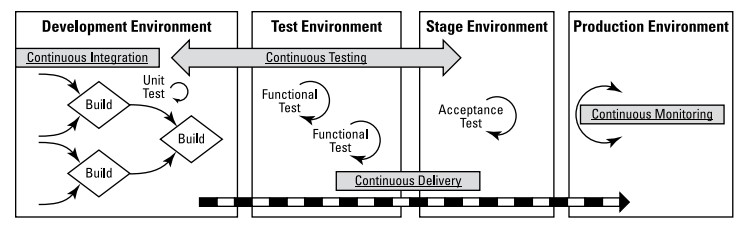
\includegraphics[scale=.7]{imagens/pipeline.jpg}
    \source{\citetexto{Humble2012}}
    \label{fig:pipeline}
\end{figure}



%\subsubsection{Integração contínua}

A \textbf{Integração contínua} é um termo oriundo da metodologia ágil  \textit{eXtreme Programming} (XP) e utilizado em diversas metodologias, que consiste em integrar código alterado e/ou desenvolvido ao projeto principal na mesma frequência com que as funcionalidades são desenvolvidas, podendo ser realizado diversas vezes ao dia, ao invés de apenas uma vez. Segundo \citetexto{Fowler2006}, a principal ideia  por trás deste processo é verificar se as alterações ou novas funcionalidades não criaram novos defeitos no projeto já existente e cada integração é verificada por um \textit{build} automatizado (incluindo testes) para detectar erros de integração o mais rápido possível, muitos times acreditam que esse tipo de abordagem leva a uma significante redução nos problemas de integração e permite que um time desenvolva \textit{software} coeso mais rapidamente.

As informações sobre \textit{builds}, testes e implantação são armazenadas em um \textit{pipeline} de implantação. Neste \textit{pipeline} de implantação, constam todos os dados referentes às fases do andamento da implantação. Para utilizar integração contínua é obrigatório adotar algumas práticas, tais como: utilizar controle de versão, usar \textit{builds} automatizados, usar estes isolados, realizar \textit{commits} diários no repositório, utilizar um servidor de integração, executar testes automatizados e testes de infraestrutura. É interessante observar que diferente da integração ``comum'', onde o software é considerado como não funcional até que a fase de testes valide que o mesmo funcione, já na integração contínua, o \textit{software} é considerado funcionado, e a cada mudança no \textit{software}, um conjunto de testes automatizados é executado para garantir seu funcionamento, permitindo assim, em caso de problemas, observar as falhas existentes de maneira mais ágil, diminuindo os prejuízos de correção.

O objetivo desta prática é resolver problemas usuais de desenvolvimento de \textit{software} de maneira mais rápida, pois integrando de maneira contínua, o processo se torna mais fluído, o que facilita na rastreabilidade de um problema. Organizações que não possuem este tipo de prática, tendem a realizar integrações após longos períodos de tempo, fazendo com que a rastreabilidade de problemas e o tempo de resolução cresça consideravelmente. Em grande parte dos casos, o servidor de integração contínua também é responsável por aplicar testes automatizados e validar os \textit{check-ins} entregues por desenvolvedores, também pode realizar testes de integração, desempenho e carga, caso o resultado destes seja positivo, a nova versão do \textit{software} pode ser disponibilizada para o ambiente de produção.

%\subsubsection{Entrega contínua}
O objetivo da prática de \textbf{entrega contínua} é permitir que novas funcionalidades de software sejam entregues para clientes e usuários da maneira mais breve possível, trata-se de uma prática complementar à integração contínua, possibilitando a criação de \textit{pipelines} de implantação automatizados \cite{Sharma2014}.

\citetexto{Humble2012} destacam que a repetitividade e confiabilidade são fundamentais para a entrega contínua de \textit{software}. Eles são obtidos através da automatização de todo processo, desde compilar e utilizar controle de versão para configuração, até a implantação e testes da aplicação, ou seja, a maior parte dos processos e práticas abordados em DevOps são direcionados para viabilizar as práticas de integração contínua e a entrega contínua de \textit{software}.

A automação é um fator crucial para esta prática, pois por meio dela, é que será possível efetuar mudanças entre estágios de criação, implantação, testes e release, realizando a mudanças entre estes como por exemplo, pressionando apenas um botão. 
Ainda para \citetexto{Humble2012}, esta prática possibilita aos times de desenvolvimento a entrega de \textit{software} em ambientes de produção de maneira previsível, confiável e com poucos riscos ao negócio. Conforme dito esta prática visa encurtar o tempo entre realizar alterações em uma aplicação e conseguir implementá-la, garantindo que possíveis falhas sejam identificadas o mais breve possível, o que torna mais fácil de corrigi-las.

\citetexto{Wotton} destacam que a entrega contínua de \textit{software} tem como por objetivo:
\begin{itemize}
\item Entregar \textit{software} de uma maneira rápida e frequente, agregando valor ao negócio e obtendo feedbacks de maneira mais breve possível;
\item Propiciar um aumento na qualidade, estabilidade  e minimizar o \textit{downtime} de aplicações;
\item Reduzir os riscos do processo de release, testando todos os produtos em ambientes de testes e ambientes semelhantes ao ambiente produtivo;
\item Reduzir o desperdício de trabalho e aumentar a eficiência no processo de desenvolvimento;
\item Entregar e manter o \textit{software} em um estado de pronto, onde é possível implantar o mesmo de acordo com as necessidades do cliente.
\end{itemize}
Ainda segundo \citetexto{Wotton}, para atingir esses objetivos é  necessário automatizar as seguintes áreas e práticas:
\begin{itemize}
\item  Compilação e empacotamento: O processo de compilação que transforma código fonte em artefatos de implantação;
\item  \textit{Builds} e Entrega Contínua: A partir da integração contínua são disparados os processos do pipeline de entrega, como testes, implantação e gerenciamento de \textit{releases};
\item Automação de testes: Usualmente realizado por um servidor de integração (CI) a cada checkin realizado por desenvolvedores. O conjunto de testes devem cobrir os mais variados níveis de abstração (unidade, integração, aceitação, carga, performance e fumaça). Os testes são distribuídos conforme a necessidade dos estágios do pipeline de implantação, com o objetivo de identificar problemas o mais breve possível;
\item Implantação automática: Implantar \textit{software} de maneira automatizada, de modo que os times possam realizar esta tarefa de maneira \textit{self-service}, implantando os sistemas sem dependências da equipe de operações. Este ponto é chave para a entrega contínua;
\item Infraestrutura Como  código: Ferramentas de gerenciamento de configuração para infraestrutura permitem definir e controlar a infraestrutura a partir de arquivos de definição em código, permitindo assim a construção de ambientes consistentes, confiáveis e reproduzíveis de maneira automática, gerando assim a base para um pipeline de implantação confiável;
\item \textit{Pipeline} de implantação: É outro ponto chave para o processo de entrega contínua, ele fornece a visibilidade necessária sobre o andamento de todo o processo de entrega nos estágios e etapas que os \textit{releases candidates} sofrem, ou seja, o caminho realizado da etapa de código fonte até a produção. Fornecem também critérios para um \textit{build} mover-se entre os estágios do pipeline e conhecimento para a tomada de decisão de acordo com os resultados obtidos.
\end{itemize}

%\subsubsection{Testes contínuos e automatizados}
Os \textbf{Testes contínuos e automatizados} são importantes levando em conta que todos os processos em DevOps produzem código para a produção, assim que a etapa de desenvolvimento é finalizada. Isso requer que o código seja continuamente integrado e em paralelo, é necessário aplicar conjunto de testes que trabalhe com a integração destas novas funcionalidades. Com implantações sendo realizadas de maneira mais rápida e frequente, é impossível executar testes manuais  de todas funcionalidades a cada release. Testar é uma atividade multifuncional que envolve todo o time e deve ser executada continuamente, durante todo o ciclo de vida do desenvolvimento. \cite{Humble2012}.  
Para \citetexto{Duvall2007} não existe integração contínua sem a implementação de testes contínuos e automatizados, pois é por meio deles que os desenvolvedores e demais partes envolvidas no processo de desenvolvimento adquirem confiança sobre as mudanças realizadas realizadas no \textit{software}.

%\subsubsection{Infraestrutura Como Código}
\textbf{Infraestrutura como um código} é uma abordagem para automação de infraestrutura baseada em práticas de desenvolvimento de \textit{software}. A ênfase desta prática é em automação de rotinas consistentes e repetitivas, para provisionamento e mudança de configurações em sistemas. As mudanças são feitas em arquivos de definição e após isso, e estas são realizadas de maneira autônoma, incluindo a validação destas alterações.
A premissa das ferramentas modernas é a de que a infraestrutura pode ser tratada exatamente como um \textit{software}.  Como resultado, todo o trabalho manual que era realizado, como por exemplo, a realização de alterações feitas diretamente em um servidor (ex: Configuração de uma variável de ambiente) deixa de ser realizado. Todas as alterações a serem realizadas devem estar em arquivos de configuração versionados em um repositório como Git ou similar, como qualquer outro código fonte. \citep{Morris2016}.

A partir destes arquivos de definição, um ambiente pode ser criado automaticamente do zero, com as mesmas características de outros ambientes da mesma versão. A qualquer momento, alguém pode olhar o histórico dos arquivos de definição e analisar as configurações do ambiente em uma determinada versão, o que de fato já pode ser considerado uma forma de ``documentação viva'' que corresponde ao exato estado do sistema naquele ponto.

Baseado neste paradigma, criar e destruir ambientes frequentemente é uma boa prática. Um dos motivos é garantir que o ambiente sempre estará consistente com a configuração descrita. Além disso, reforça a cultura de que o ambiente de execução é descartável e não deve ser considerado uma ``fonte de verdade'' (\textit{source of truth}).
Um benefícios de transformar a infraestrutura em código é a possibilidade de implementar a integração contínua de maneira adequada, permitindo a execução automática, isolada, e com testes de integração em ambientes com configurações idênticas à de produção. Também torna mais fácil o \textit{rollout} de uma aplicação do ambiente de homologação para o ambiente produtivo e como o processo é bem definido e bem descrito, podemos pensar na escalabilidade de uma aplicação em momentos de pico, de maneira automatizada. Em caso de problemas, o esforço é menor, pois para realizar o \textit{rollback} para a versão anterior da aplicação, seria necessário somente utilizar os arquivos de descrição. Como principal desvantagem, observa-se que para versionar a configuração, será exigido um tempo maior. A instalação manual de um servidor geralmente é rápida, porém, não é escalável. Já a definição da infra em arquivos de definição pode ser mais custosa, principalmente se o operador não for experiente no assunto.

\subsection{Trabalhos relacionados}
O trabalho realizado por \citetexto{Kerzazi2016} realiza o mapeamento de atividades e áreas de conhecimento consideradas importantes para profissionais que atuam como ``DevOps / \textit{Release Engineers}''. Esse mapeamento foi realizado em Setembro de 2015, a partir da análise de 211 postagens de emprego realizadas no site monster.com, considerado um dos maiores sites de anúncios de emprego no mundo. Essa análise escolheu, de maneira randômica, 119 postagens de emprego realizadas nos Estados Unidos, 33 no Canadá, 49 no Reino Unido, 6 na Austrália e 4 na índia.  De maneira resumida, os autores realizaram a análise de maneira qualitativa manual de 144 postagens, para entender melhor as responsabilidades e deveres desejados no perfil destes profissionais. Os resultados desta análise foram utilizados para a elaboração de parte do questionário deste presente estudo e também para o mapeamento de práticas, habilidades e responsabilidades destes profissionais. As perguntas \textbf{22 e 23} são compostas a partir das habilidades mapeadas por este trabalho.

Já \citetexto{Jabbari2016} apresenta um mapeamento sistemático sobre o que é DevOps, explanando suas definições e práticas. O objetivo deste trabalho era além de realizar um mapeamento das práticas associadas a DevOps, entender quais eram as diferenças entre DevOps e outros métodos de desenvolvimento de \textit{software}. Entre os achados desta pesquisa destacam-se a proposta de definição de que DevOps é uma metodologia de desenvolvimento entre equipes de Desenvolvimento e Operações, que tem como ênfase a comunicação e colaboração, integração contínua, \textit{Quality Assurance} e entrega de implantações de maneira automatizada, utilizando um conjunto de práticas de desenvolvimento de software. Ainda, entende que DevOps é uma extensão dos métodos ágeis e que práticas de desenvolvimento ágil são a base para suportar as práticas contidas em DevOps. 

\citetexto{Braga2015} realiza um panorama sobre as práticas DevOps utilizadas nas indústrias de \textit{software} brasileiras, além disso, também realiza um mapeamento sobre quais metodologias ágeis estão relacionadas às práticas de DevOps. 
\citetexto{Levita2017} teve como objetivo compreender como empresas de grande porte, que utilizam práticas de DevOps no processo de desenvolvimento de \textit{software} se organizam para atingir a agilidade desejada na implantação das suas aplicações. \citetexto{Levita2017} realizou a construção de questionários para cada grupo de atividades do framework \textbf{CALMS}, obtendo níveis de maturidade dos entrevistados em cada grupo de práticas em DevOps.

A presente pesquisa pretende realizar um survey direcionado para profissionais que trabalham em companhias que praticam ou que estão em processo de adoção da cultura DevOps, com o objetivo de mapear quais práticas de automação e colaboração estão em uso e entender o nível de maturidade sobre estas práticas nas organizações, o que acaba tornando-se um apanhado geral dos trabalhos citados acima, mas voltado para o contexto do Brasil.
Dessa forma, o trabalho pretende utilizar critérios de avaliação semelhantes aos utilizados por \citetexto{Levita2017} e \citetexto{Braga2015} no sentido de avaliar o nível de maturidade das práticas DevOps.

Os trabalhos de \citetexto{Kerzazi2016} e \citetexto{Jabbari2016} fornecem uma base sólida para o mapeamento de práticas utilizadas por profissionais atuantes nos ambientes DevOps, mas são voltados para realidades de outros países. Na presente pesquisa, busca-se entender se os pontos observados (habilidades e áreas de conhecimento) por \citetexto{Kerzazi2016} são aderentes à realidade encontrada no Brasil.

%=======================================================================
% Metodologia
%=======================================================================
\section{Metodologia}
Esta seção organiza-se nas seguintes etapas de pesquisa: (i) Delineamento de pesquisa, (ii) Definição da unidade de Análise, (iii) projeto do survey, (iv) análise de dados.

\subsection{Delineamento de pesquisa}
A metodologia empregada neste trabalho de pesquisa é um survey do tipo descritivo \cite{Miguel}. Neste tipo de survey, busca-se o entendimento da relevância de certo fenômeno, bem como descrever a distribuição do fenômeno da população, no caso deste survey, obter "Um panorama sobre experiências e práticas de profissionais em ambientes DevOps".

Os levantamentos bibliográficos necessários foram realizados através de pesquisas sobre palavras-chave envolvendo os termos ``DevOps'', ``Infraestrutura-ágil'', ``métodos ágeis'', ``entrega e integração contínua'' e ``infraestrutura-ágil'' nas fontes de pesquisa: IEEEXplore Digital Library\footnote{\url{https://ieeexplore.ieee.org}}, EBSCOHost\footnote{\url{https://search.ebscohost.com/}}, Google Scholar\footnote{\url{https://scholar.google.com.br/}} e Portal Períodico Capes\footnote{\url{https://periodicos.capes.gov.br}}.
%arrumar links e footnotes
%O objetivo primário não é desenvolvimento ou teste de teorias, mas possibilitar fornecer subsídios para a construção de teorias ou refinamentos. Desta forma, requer a definição de questões a serem endereçadas com argumentação lógica para a escolha da amostra. Tais questões seguem detalhadas na seção Projeto do Survey.

\subsection{Definição da unidade de Análise}
A unidade de análise compreende 1000 participantes dos grupos \textit{DevOps/SRE Porto Alegre}, \textit{Docker Porto Alegre} e \textit{DevOps BR} no aplicativo Telegram\footnote{\url{https://web.telegram.org}}. Grupos que promovem encontros mensais para debater sobre o tema DevOps e suas ferramentas, os participantes destes grupos também promovem palestras em eventos como o The Developer's Conference\footnote{\url{http://www.thedevelopersconference.com.br}} e DevOpsdays Porto Alegre\footnote{\url{https://devopsdays.org/events/2019-porto-alegre/welcome/}}, realizados anualmente. 

Assim, foi realizado o cálculo do tamanho da amostra considerando os seguintes parâmetros \cite{SurveyMonkey}: tamanho da população = 1000; margem de erro = 11\%; grau de confiança = 80\%. O resultado do tamanho da amostra foi de 33 participantes. A amostra é do tipo não probabilística por conveniência \cite{Freitas2010}, pois não houve distinção na escolha dos participantes presentes no grupo. 

A pesquisa foi disponibilizada de via formulário \textit{online} e enviada para 1000 profissionais. Houve um retorno de 33 respostas, sendo desconsideradas 3 respostas por não preencherem completamente todas as perguntas, delimitando a amostra de pesquisa em 30 participantes. Assim, houve uma taxa de retorno de 3\% (total de questionários válidos (30) / total de questionários enviados (1000)). Apesar do tamanho amostral ser inferior ao considerado ao ideal, o tamanho da amostra atual ainda é considerado o mínimo para que um resultado seja considerado confiável. \citetexto{Freitas2010}, observa a ``lei dos grandes números'' e exemplifica que amostras inferiores a 30 respostas, podem tanto mostrar um valor errôneo, quanto relatar a realidade que se pode comprovar.

Neste sentido é importante compreender o perfil do público-alvo, quanto ao tempo de experiência no setor de TI: 3\% tem de 1 a 2 anos, 10\% de 3 a 5 anos, 27\% de 6 a 10 anos e outros 60\% acima de 10 anos de experiência. Assim sendo 86,66\% dos participantes tem acima de 5 anos de experiência, o que qualifica a amostra com "credibilidade citada por \citetexto{Freitas2010}. Portanto, apesar da amostra abaixo do cálculo amostral ideal (33), considerando a argumentação de \citetexto{Freitas2010}, e o perfil do público-alvo, pode-se considerar a amostra de 30 respondentes como confiável, pois pode retratar uma realidade e dar credibilidade e validade ao estudo.  

\subsection{Projeto do Survey}

O projeto do Survey foi organizado em grupo de questões com finalidades distintas, conforme detalhado a seguir.

As \textbf{Questões 1 a 8}  relacionadas aos seguintes dados destes profissionais: Tempo de experiência, localidade em que trabalha, cargo e ramo de negócio de sua companhia. Enquanto as \textbf{questões 9 a 15} analisam o nível de colaboração e divisão de responsabilidades entre as equipes. Os constructos de \citetexto{Braga2015} e \citetexto{Levita2017} serviram de suporte para a elaboração destas questões.

As \textbf{questões 15 a 21} analisam o nível de maturidade relacionado as práticas DevOps realizadas por estes profissionais, práticas que foram levantadas por \citetexto{Braga2015}. Já os constructos  de \citetexto{Levita2017} foram também utilizados como suporte para elaboração das respostas e relacionamento com os níveis de maturidade propostos.

As \textbf{questões 22 e 23} analisam se as ferramentas e práticas levantadas por \citetexto{Kerzazi2016} são relevantes para os profissionais brasileiros.
Enquanto a \textbf{questão 24} analisa como estes profissionais estão se preparando em termos de estudo para este novo paradigma, bem como quais são suas fontes de informação sobre novas ferramentas e práticas. Por fim, as \textbf{questões 25 à 27} analisam a percepção destes profissionais sobre quais são as dificuldades e ganhos na adoção deste novo paradigma.

 Como base para as questões 9 a 21, elaborou-se uma escala adaptada sobre o modelo proposto por \citetexto{Isaca2012} em COBIT 5, no qual propõe um modelo de capacidade de processo definido em 5 níveis definidos abaixo: \textbf{maturidade 5 - Melhoria Contínua}: Prática em processo de melhoria contínua. Time possui excelência na realização da prática, que foi completamente assimilada na cultura da organização; \textbf{maturidade 4 - Avançado}: Prática otimizada pelo time e que se torna parte da cultura da organização. Resultados de negócio sempre visíveis pelo corpo gestor da organização; \textbf{maturidade 3 - Gerenciado}: Prática sistematizada pelo time ou organização. Resultados começam a tornar-se visíveis pela organização; \textbf{maturidade 2 - Consciente}: Prática embrionária no time ou organização. Resultados iniciais e ainda inconsistentes; \textbf{maturidade 1 - Inicial}: Ausência de práticas ou iniciativas \textit{ad hoc} realizadas isoladamente por algumas pessoas. As respostas apresentadas nessas questões estão organizadas de uma maneira \textit{top-down}, ou seja, o nível de maior maturidade é a primeira resposta da lista e o menor é a última.

 \subsection{Análise de dados}
Para análise dos dados utilizou-se parâmetros básicos da estatística descritiva como: média, moda e mediana. Esses parâmetros são observados em especial nas questões 9 à 25, onde encontram-se dois tipos de escala: uma adaptada do modelo proposto em COBIT 5 e descrita na seção de projeto do survey, que atende às questões 9 a 21. Enquanto as questões 22 a 24 utilizam um modelo de escala tipo Likert, que são descritas na seção de análise de resultados de cada pergunta.

O relatório final apresenta uma síntese da maturidade das práticas DevOps realizadas pelo grupo de profissionais pesquisados, no qual se apresenta visualmente a síntese dos dados estatísticos de maturidade. Para algumas questões em específico, optou-se pelo uso da representação da síntese dos resultados por meio de gráficos do tipo boxplot. Por meio destas representações buscou-se apresentar valores discrepantes nas respostas enviadas pelos entrevistados.

\begin{figure}[H]
    \centering
    \caption{Exemplo de box plot e as estatísticas por ele representadas}
       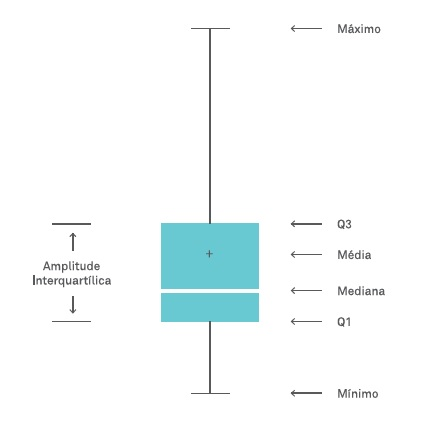
\includegraphics[scale=.6]{imagens/resumo-cinco-numeros-box-plot.jpg}
        \source{\citetexto{EDTIBoxPlot}}
       % \source{Fonte: Elaborado pelo autor}
\end{figure}

Em um boxplot são apresentadas cinco estatísticas: o mínimo, o primeiro quartil (Q1), a mediana, o terceiro quartil (Q3) e o máximo. Esses valores também são conhecidos como resumo dos cinco números.
O grande objetivo desta análise gráfica é verificar a distribuição dos dados. Assim, as possíveis conclusões são: centro dos dados (a média ou mediana), amplitude dos dados (mínimo - máximo), a simetria ou assimetria do conjunto de dados e a presença de \textit{outliers}.
No centro do quadrado, temos uma linha que indica o valor da mediana. A dispersão é representada pela amplitude do gráfico, que pode ser calculada como valor máximo ou mínimo. Quanto maior for a amplitude, maior a variação dos dados.
O retângulo contém 50\% dos valores do conjunto de dados. A posição da linha mediana no retângulo informa sobre a assimetria da distribuição. Quando uma distribuição é considerada simétrica, a mediana ocupa o centro do retângulo. Caso o valor da mediana esteja mais próximo de Q1, os valores são positivamente assimétricos. Caso sejam mais próximos de Q3, são negativamente assimétricos \cite{EDTIBoxPlot}.

\section{Uma análise sobre o panorama de experiências profissionais em ambientes DevOps}
Nesta seção realiza-se a análise dos resultados do Survey e subdivide-se da seguinte forma: (a) dados sócio-demográficos, (b) Análise de maturidade sobre práticas DevOps, (c) ferramentas e atividades, (d) fontes de informação, e (e) dados qualitativos sobre dificuldades e ganhos na adoção do DevOps.

\subsection{Dados sócio-demográficos}
O público alvo desta pesquisa é composto por profissionais da área de Desenvolvimento e Operações de companhias que praticam ou estão em fase de adoção da cultura DevOps. Observa-se na Figura \ref{fig:cargos} que 30\% dos entrevistados estão atualmente trabalhando como Desenvolvedores de Software e outros 20\% na área de Infraestrutura de TI.  Cabe destacar que 6,67\% dos profissionais optaram por não declarar seu cargo. Essa questão foi considerada opcional, com a intenção de não afastar possíveis respondentes que de alguma forma poderiam sentir-se de desconfortáveis em relação ao sigilo da pesquisa. 
\begin{figure}[H]
    \centering
    \caption{Cargo dos entrevistados}
       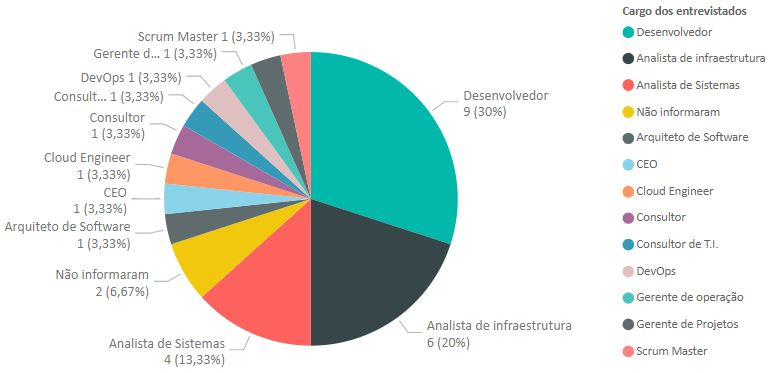
\includegraphics[scale=.6]{imagens/cargos_pbi.JPG}
       \source{Elaborado pelo autor.}
    \label{fig:cargos}
\end{figure}
Observa-se na Figura \ref{fig:experiencias} que quando questionados sobre qual seria seu campo de experiência predominante, ou seja, na área em que atuou por um maior período de tempo, 63,3\% dos entrevistados respondeu que suas experiências estão predominantemente ligadas à área de desenvolvimento de \textit{software} (Desenvolvimento de \textit{software} (\textit{Front-End, Back-End}, Testes, \textit{Mobile}, etc.), outros 23,33\% ligados à infraestrutura de TI (Banco de dados, \textit{Middleware}, Infraestrutura, Serviços, etc..).

\begin{figure}[H]
    \centering
       \caption{Resumo de experiências dos entrevistados}
       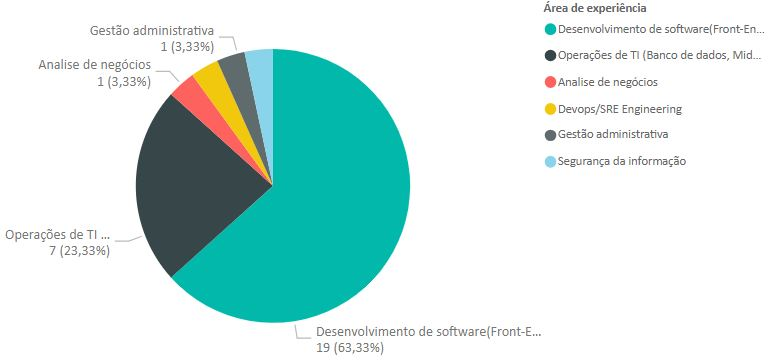
\includegraphics[scale=.6]{imagens/exp_pbi.jpg}
      \source{Elaborado pelo autor.}
    \label{fig:experiencias}
\end{figure}

Na Figura \ref{fig:expAns} observa-se que 60\% dos entrevistados possui mais de 10 anos de experiência na área de TI, bem como outros 26,67\% possui entre 6 a 10 anos de experiência. Quando indagados sobre o tempo de experiência gerenciando/utilizando ferramentas de automação voltadas para DevOps, nota-se que 43,33\% dos entrevistados possuem de 1 a 2 anos de experiência e apenas 13,33\% está ainda em fase de pesquisa sobre ferramentas de apoio utilizadas em DevOps. 

\begin{figure}[H]
    \centering
     \caption{Resumo de experiências profissionais (Em anos)}
     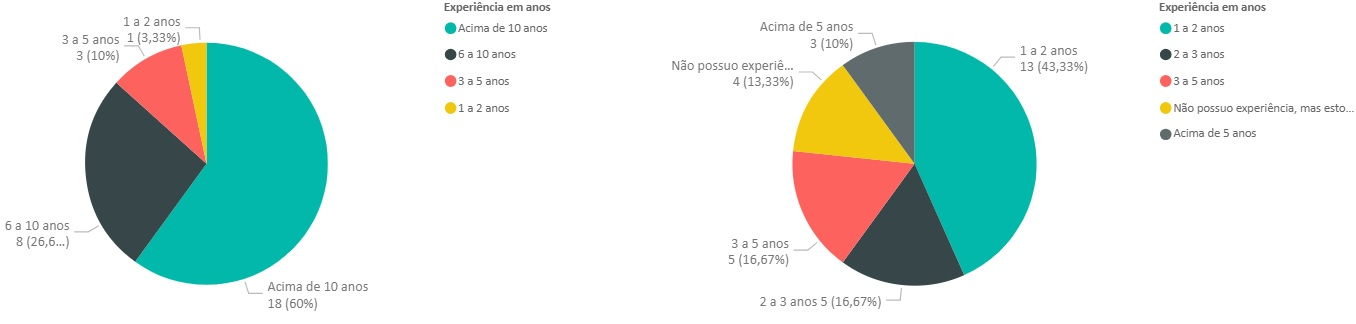
\includegraphics[scale=.5]{imagens/tempoExperiencia_pbi.jpg}
     \source{Elaborado pelo autor.}
    \label{fig:expAns}
\end{figure}

Para classificar o porte das empresas e outras informações, o Sebrae utiliza como base pesquisas divulgadas pelo Instituto Brasileiro de Geografia e Estatística (IBGE) conforme o número de empregados: micro, pequena, média e grande empresa. \citep{SEBRAE2017}. 
Conforme a Figura \ref{fig:PorteEmpresas}, observa-se que 53\% dos entrevistados trabalham em empresas classificadas como grandes, 16,67 \% em médias,  também 16,67\% em micro e os 13,33\% restantes em pequenas empresas. 

\begin{figure}[H]
    \centering
    \caption{Porte das empresas}
       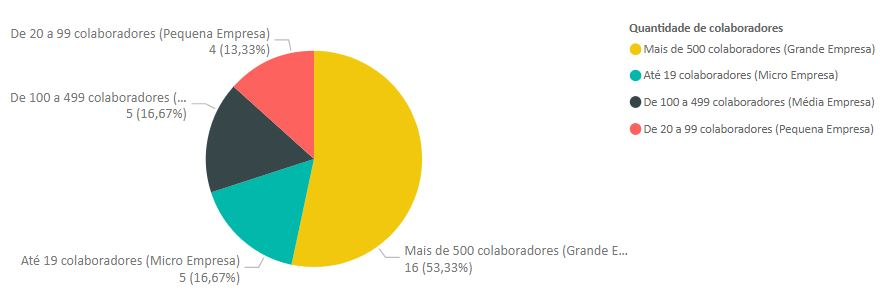
\includegraphics[scale=.6]{imagens/colaboradores_pbi.JPG}
        \source{Elaborado pelo autor.}
     \label{fig:PorteEmpresas}
    \end{figure}

A Figura \ref{fig:colaboradores} apresenta a distribuição das empresas por atividade econômica. Observa-se que 46,67\% dos entrevistados estão relacionados à empresas de tecnologia/produção de software e outros 20\% estão relacionados à empresas de serviços financeiros. Os demais entrevistados estão divididos entre as mais diversas atividades, como Educação, Orgãos governamentais, Varejo e Comércio, etc.

\begin{figure}[H]
    \centering
    \caption{Atividade Econômica}
       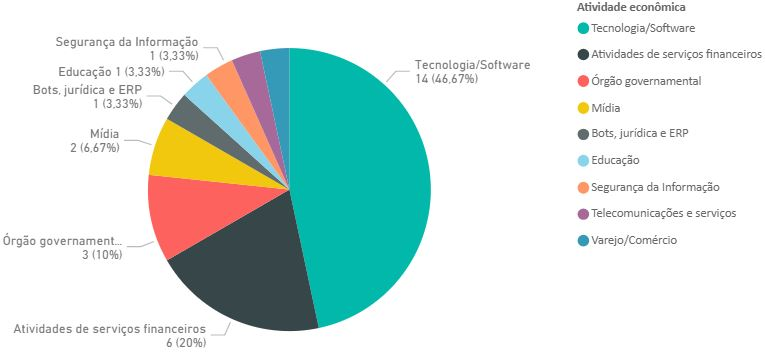
\includegraphics[scale=.6]{imagens/atividadeEcon_PBI.JPG}
        \source{Elaborado pelo autor.}
    \label{fig:colaboradores}
\end{figure}

\subsection{Análise sobre o nível de colaboração entre as equipes de Desenvolvimento e Operações.}

Esta seção realiza uma análise individual das questões 9 a 15. Esses questionamentos visam entender em que estágio de maturidade está o compartilhamento de tarefas, ferramentas, oportunidades e responsabilidades entre as equipes. \textcolor{red}{No final desta seção é realizada uma síntese com os valores médios de maturidade para cada questão analisada.} Nas representações gráficas utilizou-se uma escala de cores para representação dos níveis de maturidade, afim de facilitar a conexão entre os níveis de maturidade e a visualização de dados nos gráficos gráficos. Classificam-se as cores da seguinte maneira: {\textcolor{yellow}{Amarelo}} - Nível de maturidade 5; \textcolor{persiangreen}{Verde} - Nível de maturidade 4; \textcolor{gray}{Cinza} - Nível de maturidade 3; \textcolor{red}{Vermelho} - Nível de maturidade 2; \textcolor{orange}{Laranja} - Nível de maturidade 1.\\ \indent
 A Figura \ref{fig:crossFuncionais} apresenta os resultados da questão 9, observa-se que grande parte dos entrevistados já trabalha (ao menos em alguns projetos), em um time cross-funcional. A ideia por trás desta prática e quebrar as barreiras existentes entre os times e sistematizar o sentimento de que todos os indivíduos são responsáveis pelo processo de entrega.
Apenas sete (23,33\%) dos entrevistados ainda não trabalha desta forma. 
Algumas organizações denominam estes times como \textit{Squad} ("Esquadra"). Muitas empresas se inspiram no modelo proposto \citetexto{SPOTIFY}, onde cada squad funciona como uma mini-startup. A equipe é auto-organizada e possui autonomia suficiente para decidir seus processos internos.

\begin{figure}[H]
    \centering
    \caption{Sua organização trabalha com times cross-funcionais?}
       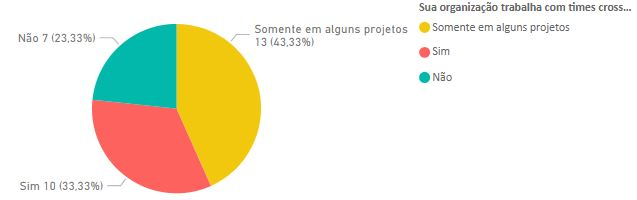
\includegraphics[scale=.63]{imagens/crossFuncionais_PBI.JPG}
        \source{Elaborado pelo autor.}
    \label{fig:crossFuncionais}
\end{figure}
%\subsubsection{Compartilhamento de conhecimento entre os times}
A questão 10 tem como objetivo analisar o quanto os times compartilham suas informações. Na Figura \ref{fig:compartConhecimento} é possível observar que na organização para 14 (46,67\%) dos entrevistados as informações são compartilhadas apenas quando requisitado, para 11 (36,67 \%) dos entrevistados as informações estão disponíveis para todos e em formatos dinâmicos, como \textit{Wikis} e salas de bate-papo (plataformas como Slack e MS Teams). 
A questão 10 está diretamente ligada ao \textbf{S - Sharing} do framework CALMS e visa entender o quão dinâmica e sem obstruções é a comunicação entre os times. 
\newline
\begin{figure}[H]
    \centering
    \caption{Como você descreveria o compartilhamento de conhecimento entre times?}
       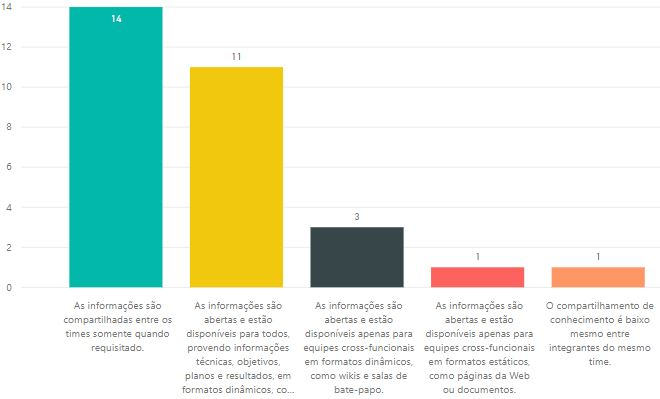
\includegraphics[scale=.6]{imagens/compartilhamentoConhecimento.JPG}
        \source{Elaborado pelo autor.}
    \label{fig:compartConhecimento}
\end{figure}
%
%\subsubsection{Compartilhamento de ferramentas entre Dev e Ops}
Na Figura \ref{fig:compartFerramentas} observa-se que 14 (46,67\%) dos entrevistados ainda realiza o compartilhamento de ferramentas de forma parcial, enquanto outros sete (23,33\%) possuem suas ferramentas integradas, mas não possuem um fluxo único de entrega. Apenas quatro (13,33\%) dos entrevistados possuem um fluxo único de entrega e com todas as suas ferramentas integradas, outros três (10\%) compartilham algum status entre suas ferramentas via monitoramentos e apenas para dois (6,66\%) usam ferramentas totalmente distintas para suas tarefas.

Embora o foco em DevOps seja o mesmo que o descrito no manifesto ágil (Indivíduos e interações em detrimento a processos e ferramentas), ter um conjunto único de ferramentas que forme de fato uma ``esteira'' de entrega de software pode otimizar a entrega e diminuir a pressão constante entre os times.

\begin{figure}[H]
    \centering
    \caption{Compartilhamento de ferramentas entre os times de Dev e Ops}
       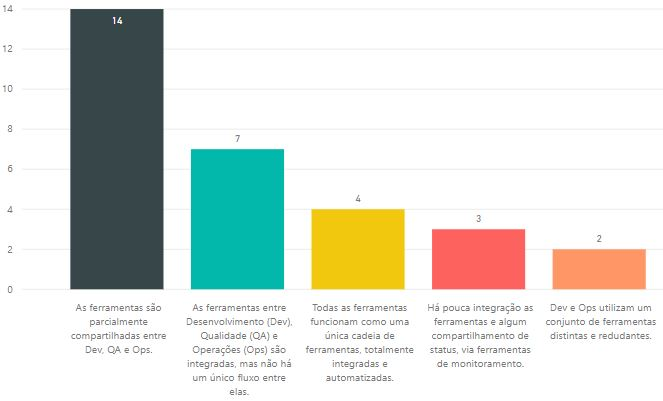
\includegraphics[scale=.6]{imagens/compartilhamentoFerramentas.JPG}
        \source{Elaborado pelo autor.}
    \label{fig:compartFerramentas}
\end{figure}

Quando questionados sobre o processo de levantamento de requisitos não-funcionais, observa-se que 11 (36,67\%) dos entrevistados entende que esta é uma responsabilidade de ambas as equipes, porém, estes dados não são levados em conta durante o processo de desenvolvimento e que, 10 (30\%) realiza o levantamento de todos os requisitos ao longo do processo de desenvolvimento, porém, o time de operações não é incluído nas discussões. 
\begin{figure}[H]
    \centering
    \caption{A equipe de desenvolvimento considera requisitos não-funcionais no processo de desenvolvimento de uma aplicação?}
       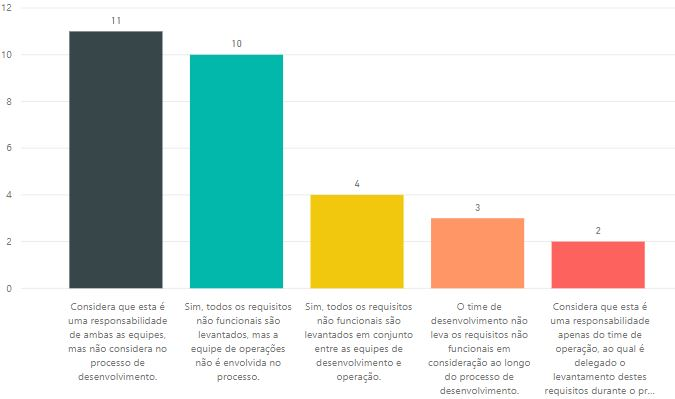
\includegraphics[scale=.6]{imagens/requisitos.JPG}
        \source{Elaborado pelo autor.}
    \label{fig:requisitos}
\end{figure}

%\subsubsection{Colaboração, divisão de riscos, inovação e aprendizado}
Quando questionados sobre o nível de colaboração entre os times, observa-se que os entrevistados encontram-se bem distribuídos entre os níveis de maturidade propostos. A partir da Figura \ref{fig:colaboracaoInovacao}, percebe-se que dez (30\%) deles já atingiram o nível de melhoria contínua neste quesito, já oito (26,67\%) estão no nível avançado e outros cinco (20\%) estão em um nível gerenciado. 

\begin{figure}[H]
    \centering
        \caption{Como o seu time colabora, divide riscos, inova e aprende?}
       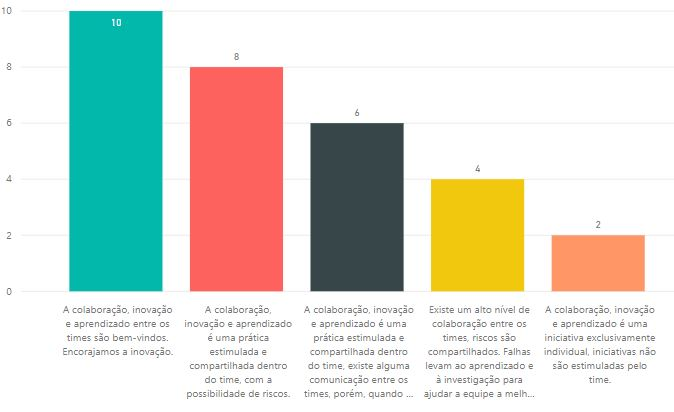
\includegraphics[scale=.6]{imagens/colaboracaoInovacao.JPG}
        \source{Elaborado pelo autor.}
    \label{fig:colaboracaoInovacao}
 \end{figure}
%\subsubsection{Planejamento, priorização e agendamento do trabalho}
Ainda seguindo na linha de divisão de responsabilidades, os entrevistados responderam sobre como o trabalho é planejado, priorizado e agendado dentro de suas companhias. Observa-se na Figura \ref{fig:planejamentoTrabalho} que as respostas não acompanham a tendência em relação a questão de colaboração, 12 (40\%) dos entrevistados dizem que há uma tentativa de priorização de trabalho dentro das equipes, mas de maneira irregular. 

\begin{figure}[H]
    \centering
    \caption{Como é planejado, priorizado e agendado o trabalho?}
       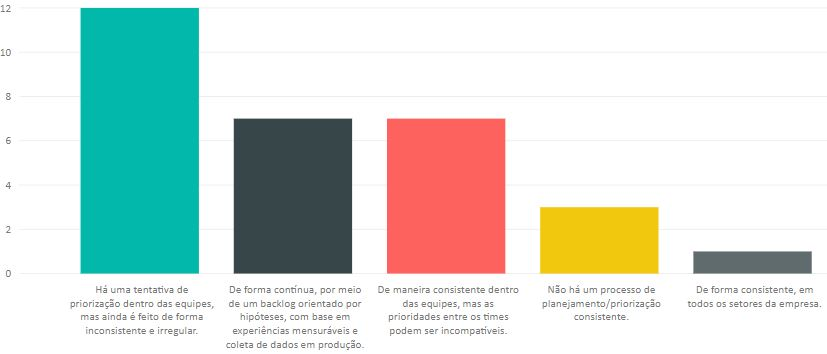
\includegraphics[scale=.6]{imagens/priorizacao.JPG}
        \source{Elaborado pelo autor.}
    \label{fig:planejamentoTrabalho}
\end{figure}

Observa-se neste item que apesar dos entrevistados responderem que possuem um alto nível de colaboração entre as equipes, ainda não há um processo bem estabelecido quanto ao planejamento de trabalho. Ponto que pode causar desconfortos entre os times quanto a definição de prioridades em suas rotinas.

\subsection{Análise de maturidade sobre práticas DevOps}
Realiza-se nesta seção uma análise sobre o nível de maturidade das técnicas de automação utilizadas em DevOps. Analisa-se em particular as técnicas de Infraestrutura-como-Código, Monitoramento Contínuo, Entrega/Integração Contínua, Testes Contínuos e Melhoria Continua. Para tanto, utilizamos a escala citada no seção de Projeto do Survey.  Cabe destacar que esta pesquisa considera uma amostra de análise, ou seja, os dados analisados apontam para o nível de maturidade de uma determinada amostra de profissionais inseridos em companhias que praticam a cultura DevOps e suas práticas de automação.

A Tabela 1 apresenta os resultados obtidos nas questões 14, 16, 18, 19, 20 e 21. Segundo os resultados, observa-se que grande parte dos entrevistados ainda estão entre os níveis de maturidade inicial e gerenciado em relação as práticas de automação.
\setlength{\belowcaptionskip}{0.0pt}
\begin{table}[H]
\footnotesize
\caption{Distribuição dos níveis de maturidade}
    \begin{tabularx}{\columnwidth}{cccccc}
    \hline
       Prática                  &    Inicial &    Consciente &    Gerenciado &    Avançado &    Melhoria contínua \\ \hline 
       Infra-Como-Código        &    6 (20,00\%)  &    11 (36,67\%)    &    4 (13,33\%)    &    6 (20,00\%)  &    3 (10,00\%)           \\
       Testes   contínuos       &    11 (36,67\%) &    3 (10,00\%)    &    7 (23,33\%)    &    3 (10,00\%)  &    6 (20,00\%)           \\
       Integração   contínua    &    5 (16,67\%)  &    7 (23,33\%)    &    11 (36,67\%)    &    4 (13,33\%)  &    3 (10,00\%)           \\
       Entrega   contínua       &    6 (20,00\%) &    6 (20,00\%)    &    8 (26,67\%)    &    7 (23,33\%)  &    3 (10,00\%)           \\ 
       Monitoramento   contínuo &    3 (10,00\%) &    9 (30,00\%)    &    7 (23,33\%)    &    7 (20,00\%)  &    3 (16,67\%)           \\
       Melhoria   contínua      &    4 (13,33\%) &    13 (43,33\%)    &    4 (13,33\%)    &    5 (16,67\%)  &    4 (13,33\%)           \\ \hline
    \end{tabularx}
    \source{Elaborado pelo autor.}
\end{table}

Observa-se na Figura \ref{fig:pratDevOps} que o nível médio de maturidade em geral é igual a \textbf{2,77}, ou seja, em média os entrevistados estão se aproximando ao correspondente ao nível \textbf{gerenciado}. Pode se concluir que as práticas estão sendo sistematizadas pelo time ou organização e os resultados começaram a tornar-se visíveis pela organização. Observa-se também na Figura \ref{fig:pratDevOps} os valores para média, moda e mediana para cada prática. 
\begin{figure}[H]
    \centering
    \caption{Análise sobre as práticas DevOps}
       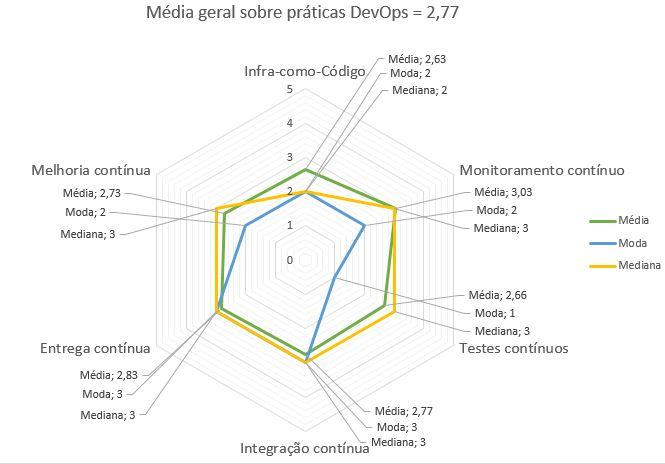
\includegraphics[scale=.6]{imagens/maturidade_radar.JPG}
        \source{Elaborado pelo autor.}
    \label{fig:pratDevOps}
\end{figure}

Cabe lembrar que podem existir distorções de análise, principalmente quando existem resultados extremos de uma escala.

%\subsection{Análise sobre a opinião dos profissionais}
\subsection{Analise da percepção sobre a adoção da cultura DevOps}

Nesta seção é realiza-se uma análise sobre as questões 22 à 27. Esta seção é sub-dividida em três partes: (I) Análise sobre relevância de conjuntos de ferramentas voltadas para DevOps, (II) Análise sobre como estes profissionais estão se preparando em termos de estudo para este novo paradigma, (III) Os principais benefícios e dificuldades, segundo a percepção dos profissionais.
\subsubsection{Análise sobre as ferramentas e atividades em DevOps}
Nas questões 22 e 23 utiliza-se uma escala de um à cinco, onde 1 = Sem importância e 5 = Muito importante.
Observa-se na Figura \ref{fig:importanciapratDevOps} que as atividades consideradas \textit{core} mapeadas por \citetexto{Kerzazi2016} são de fato consideradas relevantes para os entrevistados. Optou-se pela apresentação dos resultados em um gráfico em formato de boxplot pela facilidade na análise dos resultados. A partir desta representação gráfica percebe-se que há uma grande variação entre os níveis Razoavelmente importante / Muito importante nas respostas dos entrevistados. Em geral, o valor mediano das respostas classificou as ferramentas como Importantes. Também é possível observar que os tópicos de que são classificados como mais importantes são os tópicos de monitoramento e integração (Controle de códigos fonte, estratégias de branch..). 
Este tipo de apresentação também facilita a detecção de valores discrepantes em relação às demais respostas. Conforme observa-se na Figura \ref{fig:importanciapratDevOps} existem \textit{outliers} para as seguintes práticas: Controle de código fonte (Uma resposta com nota 1), Monitoramento (Uma resposta com nota 2) e Otimização de pipelines (Uma resposta com valor 1).

\begin{figure}[H]
    \centering
    \caption{Importância das atividades segundo entrevistados}
       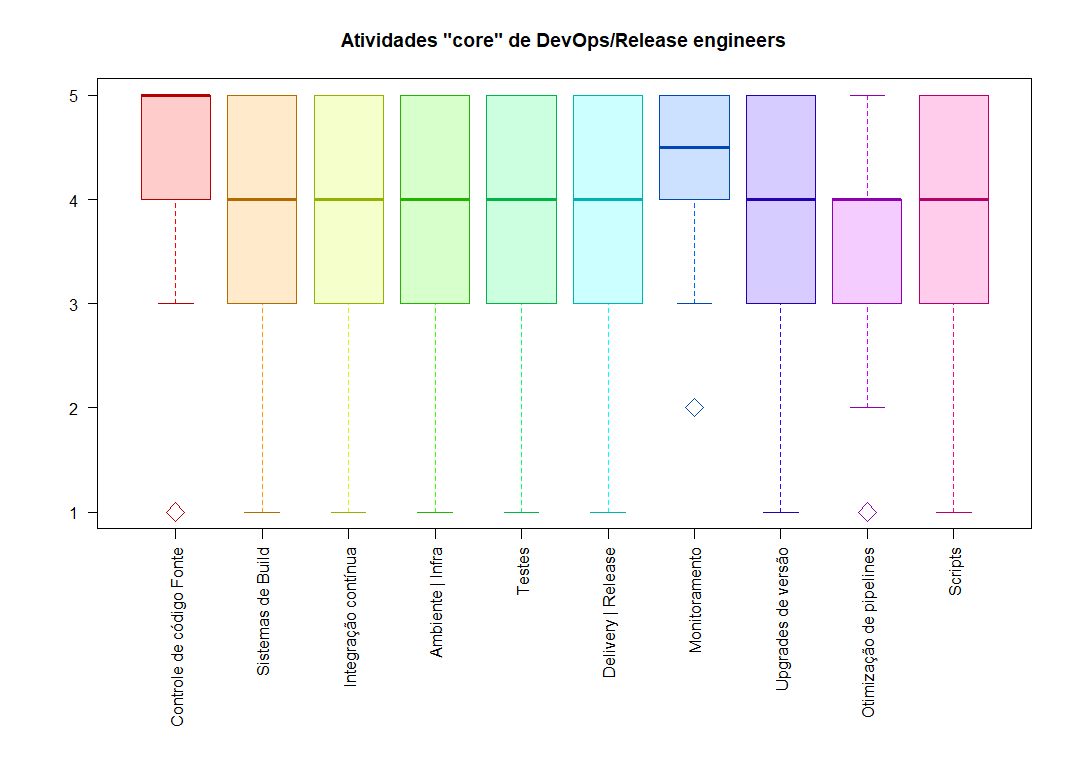
\includegraphics[scale=.5]{imagens/Rplot.png}
        \source{Elaborado pelo autor.}
    \label{fig:importanciapratDevOps}
\end{figure}
Observa-se na Figura \ref{fig:importFerramentas} que os grupos de ferramentas também mapeados por \citetexto{Kerzazi2016} também são relevantes, segundo a percepção dos entrevistados. Os grupos de ferramentas referentes à controle de versões (código), gestão de configuração, Sistemas de Build, teste e integração foram os itens que em média, possuem uma maior relevância para os entrevistados. Ferramentas de gestão de mudanças, orquestração e provisionamento, também são consideradas relevantes, porém com uma maior variância entre os níveis Sem importância e Importante.
\begin{figure}[H]
    \centering
    \caption{Importância de grupos de ferramentas segundo entrevistados}
       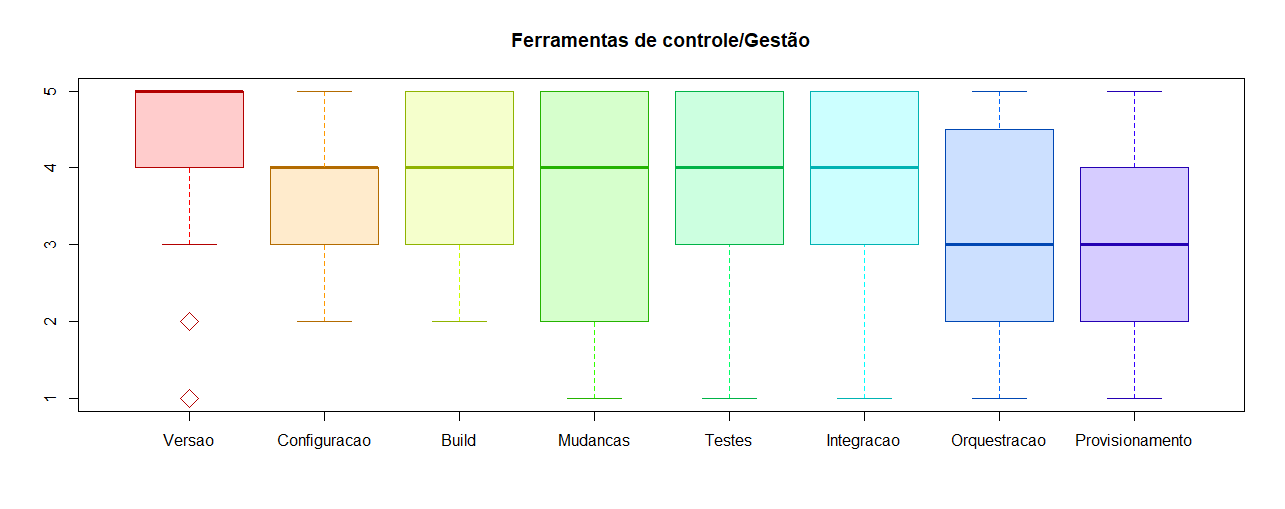
\includegraphics[scale=.5]{imagens/Rplot05.png}
        \source{Elaborado pelo autor.}
    \label{fig:importFerramentas}
\end{figure}

\subsubsection{Quais são os recursos  utilizados por estes profissionais para adquirir novos conhecimentos?}
A pergunta \textbf{24} tem como tem como objetivo realizar uma breve análise sobre quais são as principais fontes de informação utilizadas por profissionais para aprendizagem sobre o tópico DevOps. Observa-se na Figura \ref{fig:fontesConhecimento} que segundo os entrevistados, as fontes de busca sobre o assunto estão prioritariamente relacionadas a conteúdos online, como youtube, blogs técnicos, fóruns (Stack overflow,  Reddit, etc..) bem como sites de treinamentos Online. Enquanto opções como cursos presenciais e faculdade possuem uma menor adesão. Os dados brutos sobre cada tópico encontram-se na seção de anexos.
\begin{figure}[H]
    \centering
    \caption{Fontes de informação sobre DevOps}
       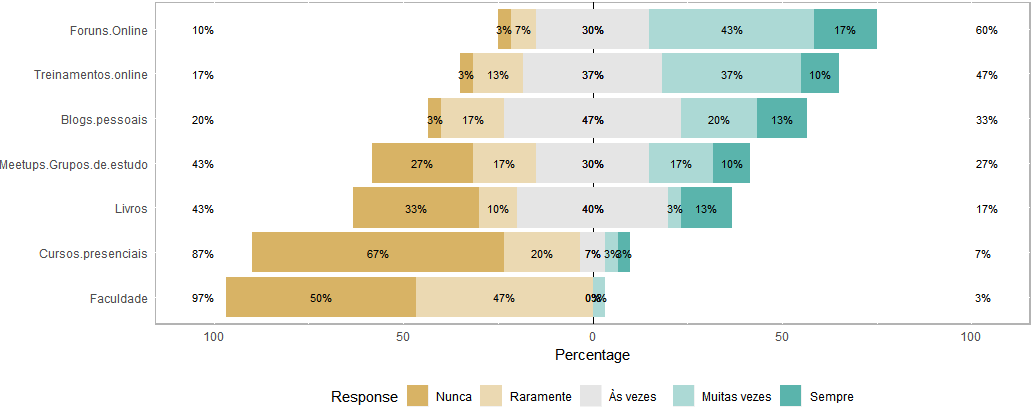
\includegraphics[scale=.5]{imagens/questao24.png}
       \source{Elaborado pelo autor.}
    \label{fig:fontesConhecimento}
\end{figure}
\subsubsection{Principais benefícios, dificuldades e opiniões sobre a cultura DevOps}
Nesta subseção analisa-se os resultados obtidos nas questões 25, 26 e 27. O objetivo destas questões é entender, segundo o ponto de vista dos entrevistados, quais são os principais benefícios, desafios e razões para não adotar a cultura DevOps. Para tanto,  uma questão baseada rankeamento foi utilizada  (questão 25). Baseados nos benefícios levantados por \citetexto{Braga2015}, foi elaborada uma série de possíveis respostas e solicitado aos entrevistados que elencassem do benefício mais importante ao menos importante. Na Figura \ref{fig:AnaliseRanking} observa-se os resultados.
\begin{figure}[!ht]
    \centering
    \caption{Principais benefícios ao adotar a cultura DevOps}
       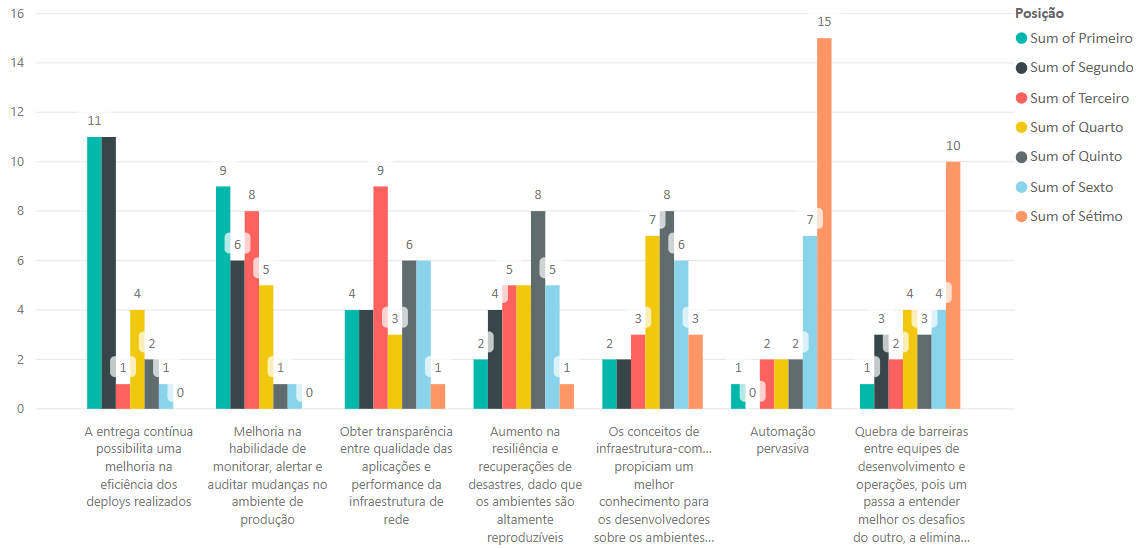
\includegraphics[scale=.6]{imagens/questao25.png}
        \source{Elaborado pelo autor.}
        \label{fig:AnaliseRanking}
       % \source{Fonte: Elaborado pelo autor}
\end{figure}
 Observa-se que segundo os entrevistados o item de Entrega Contínua é o maior benefício ao adotar a cultura DevOps. Esse item obteve 11 votos para a primeira e 11 para segunda colocação. Como terceiro colocado está a possibilidade de obter qualidade das aplicações e performance da infraestrutura de rede.
 
Já as perguntas 26 e 27 são questões abertas e que foram qualitativamente analisadas. Na questão 26 os entrevistados são questionados sobre as principais dificuldades encontradas ao iniciar a prática da cultura DevOps e na questão 27 são questionados sobre quais motivos os fariam não adotar a cultura DevOps.

Em uma breve análise qualitativa é possível observar que como principais dificuldades ao iniciar a prática da cultura DevOps estão os desafios técnicos em dominar os conjuntos de ferramentas, bem como a quebra de barreiras culturais dentro (ou silos funcionais) dentro das companhias. Como frases principais frases observa-se: ``Falta de apoio de lideranças'', ``Curva de aprendizado ou dificuldades de encontrar materiais / profissionais no Brasil'' e ``Barreiras culturais''. 

Os motivos que impediriam a adoção da cultura DevOps estão relacionados à tópicos como valores a serem investidos e, novamente, as barreiras culturais. Como principais frases observa-se: ``Falta de interesse/vontade'' e ``Falta de apoio/recursos por parte de lideranças''. As respostas na integra encontram-se na seção de anexos.

%Dada a baixa adesão destas duas questões, tornou-se inviável realizar uma análise mais profunda sobre estes dois tópicos.
\section{Discussão sobre os resultados}
Observa-se após a análise dos dados sócio demográficos que 19 (63,33\%) dos entrevistados são oriundos da área de Desenvolvimento de \textit{software} e, que 18 (60\%) dos entrevistados possui mais de 10 anos de experiência no mercado de TI. Ainda sobre os dados demográficos, observa-se que 14 (46,67\%) atualmente trabalha em companhias de Tecnologia/Software e que 16 (53,33\%) são de grandes companhias (mais de 500 colaboradores).
Na análise de perguntas relacionadas às escalas de maturidade, verificou-se que grande parte dos entrevistados distribui-se entre os níveis de maturidade consciente e gerenciado, o que significa que as práticas estão tornando-se sistematizadas dentro das organizações.
Com a análise dos dados nas questões 22 e 23 foi possível concluir que os achados de \citetexto{Kerzazi2016} sobre Ferramentas e Atividades em DevOps, são também relevantes para a realidade dos profissionais Brasileiros, segundo a percepção dos entrevistados. 
Na questão 24 realizamos uma breve análise sobre quais são as fontes de informação utilizadas pelos entrevistados para apredizagem sobre DevOps. Observa-se que em média, os entrevistados tem optado por recursos \textit{Online} em detrimento à fontes como cursos presenciais.
Na questão 25, observa-se que segundo a percepção dos entrevistados, a entrega contínua é o maior benefício ao adotar práticas DevOps dentro das possibilidades listadas na questão. 
Nas questões 26 e 27 são listados como maior desafio para iniciar em DevOps está ``Falta de apoio/interesse de lideranças/equipes'', resultado que também é observado dentre os motivos que impediriam a adoção da cultura DevOps. 


\section{Conclusão}
Este estudo propôs-se a realizar um panorama sobre o nível de maturidade das práticas DevOps para profissionais brasileiros. Para tanto, buscou-se estudos relacionados ao tema DevOps, delimitando quais são suas práticas de automação, atividades e grupos de ferramentas relacionadas ao cotidiano dos profissionais. Os achados de pesquisa forneceram uma base sólida para a construção do presente trabalho. O Survey construído para esta pesquisa com base nos achados, os termos técnicos e processos descritos são similares aos dos demais artigos afim de confirmar a validade das proposições. A análise dos dados propiciou um entendimento de que a realidade dos respondentes é muito próxima aos achados de pesquisa, validando a relevância de experiências, ferramentas e processos, bem como verificou que grande parte dos entrevistados distribui-se entre os níveis de maturidade consciente e gerenciado, o que significa que as práticas estão tornando-se sistematizadas dentro das organizações.

Para trabalhos futuros, recomenda-se a ampliação da amostra de pesquisa, afim de garantir-se um rigor estatístico, além dos parâmetros utilizados por esta pequisa. Com uma amostra maior, torna-se possível realizar uma reflexão mais profunda sobre o nível de maturidade em relação ao tempo de experiência dos entrevistados.

%=======================================================================
% Resumo em língua estrangeira (sim, é aqui mesmo).
%



% O idioma usado aqui deve necessariamente aparecer nos parâmetros do
% \documentclass, no início do documento.
%=======================================================================


%=======================================================================
% Referências
%=======================================================================


\bibliography{TCC_DevOps}


\appendix
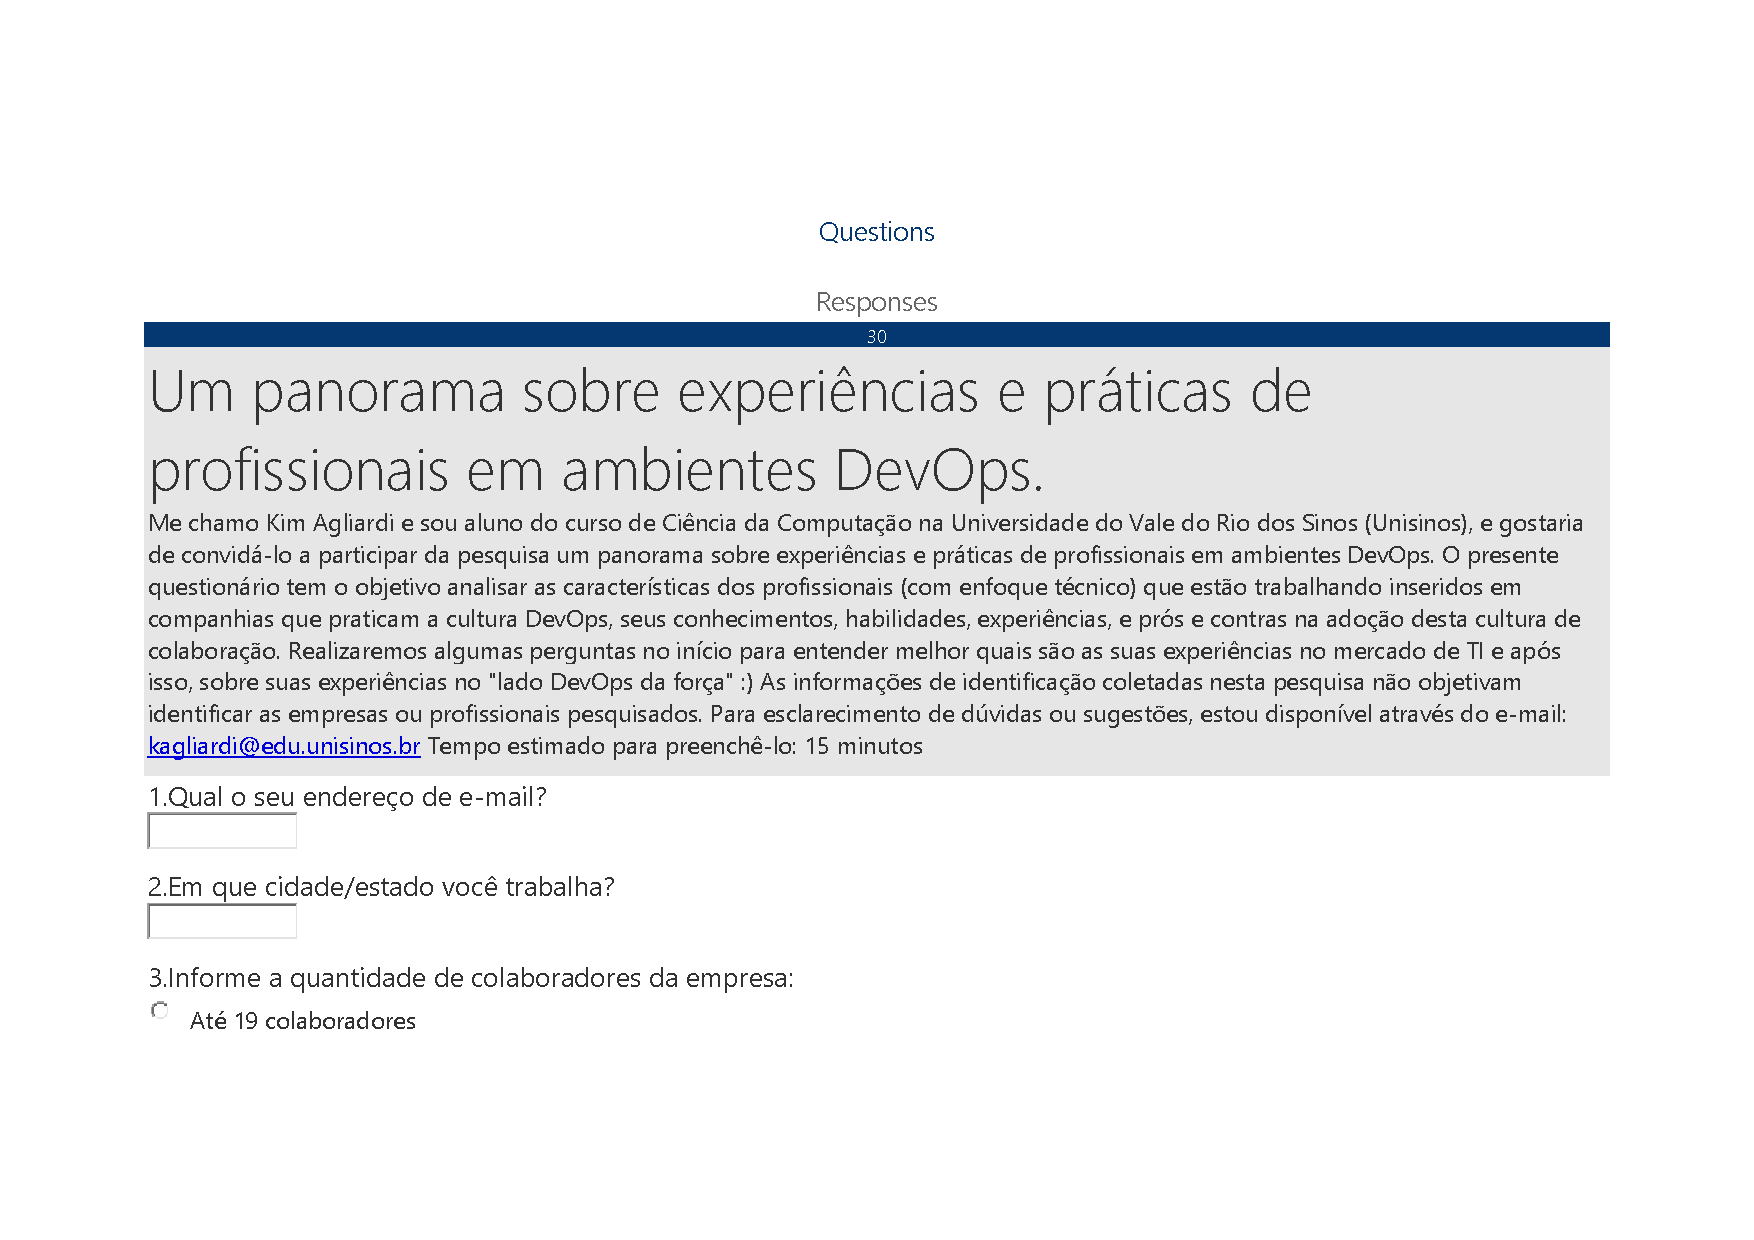
\includepdf[scale=0.8, nup = 1x3, pages=-, pagecommand=\section{Survey}]{questionario.pdf}


\section{Resultados do Survey}

\begin{table}[h]
\tiny
    \caption{Valores brutos para as questõs 1 à 4}
    \begin{tabularx}{\columnwidth}{cccccc}
    \hline
~ & ID & q1 & q2 & q3 & q4 \\
~ & 1 & fmenegussi@edu.unisinos.br & São Leopoldo/RS & De 100 a 499 colaboradores (Média Empresa) & Desenvolvimento de software(Front-End, Back-End, Testes, Mobile, etc..) \\
~ & 2 & marcelo@tisafe.com & Rio de Janeiro/RJ & De 20 a 99 colaboradores (Pequena Empresa) & Segurança da informação \\
~ & 3 & rodrigochurrops@gmail.com & São Paulo /SP & De 20 a 99 colaboradores (Pequena Empresa) & Operações de TI (Banco de dados, Middleware, Infraestrutura, Serviços, etc..) \\
~ & 4 & glauberrs@gmail.com & Porto Alegre/RS & Mais de 500 colaboradores (Grande Empresa) & Desenvolvimento de software(Front-End, Back-End, Testes, Mobile, etc..) \\
~ & 5 & Não respondeu & Porto Alegre/RS & Mais de 500 colaboradores (Grande Empresa) & Desenvolvimento de software(Front-End, Back-End, Testes, Mobile, etc..) \\
~ & 6 & andre_tocchetto@gmail.com & Porto Alegre/RS & Mais de 500 colaboradores (Grande Empresa) & Desenvolvimento de software(Front-End, Back-End, Testes, Mobile, etc..) \\
~ & 7 & Não respondeu & Porto Alegre/RS & Mais de 500 colaboradores (Grande Empresa) & Desenvolvimento de software(Front-End, Back-End, Testes, Mobile, etc..) \\
~ & 8 & berggevist@gmail.com & Porto Alegre/RS & Até 19 colaboradores (Micro Empresa) & Desenvolvimento de software(Front-End, Back-End, Testes, Mobile, etc..) \\
~ & 9 & Não respondeu & Optou por não informar. & De 100 a 499 colaboradores (Média Empresa) & Desenvolvimento de software(Front-End, Back-End, Testes, Mobile, etc..) \\
~ & 10 & jr.miranda@outlook.com  & Remoto  & Até 19 colaboradores (Micro Empresa) & Desenvolvimento de software(Front-End, Back-End, Testes, Mobile, etc..) \\
~ & 11 & diego.fl.duarte@gmail.com & Belo Horizonte/BH & De 100 a 499 colaboradores (Média Empresa) & Devops/SRE Engineering \\
~ & 12 & Ronan.vargas@gmail.com & Gravataí/RS & Mais de 500 colaboradores (Grande Empresa) & Desenvolvimento de software(Front-End, Back-End, Testes, Mobile, etc..) \\
~ & 13 & bruno_bauer@sicredi.com.br & Porto Alegre/RS & Mais de 500 colaboradores (Grande Empresa) & Desenvolvimento de software(Front-End, Back-End, Testes, Mobile, etc..) \\
~ & 14 & gfkauer@gmail.com & Porto, Portugal & Mais de 500 colaboradores (Grande Empresa) & Desenvolvimento de software(Front-End, Back-End, Testes, Mobile, etc..) \\
~ & 15 & allan@allanmoraes.com.br & Porto Alegre/RS & De 100 a 499 colaboradores (Média Empresa) & Operações de TI (Banco de dados, Middleware, Infraestrutura, Serviços, etc..) \\
~ & 16 & Não respondeu & São paulo/SP & Mais de 500 colaboradores (Grande Empresa) & Desenvolvimento de software(Front-End, Back-End, Testes, Mobile, etc..) \\
~ & 17 & diegorosa@diegorosa.com.br & Porto Alegre/RS & Mais de 500 colaboradores (Grande Empresa) & Operações de TI (Banco de dados, Middleware, Infraestrutura, Serviços, etc..) \\
~ & 18 & mesquita.cob@gmail.com & Porto Alegre/RS & Mais de 500 colaboradores (Grande Empresa) & Desenvolvimento de software(Front-End, Back-End, Testes, Mobile, etc..) \\
~ & 19 & adrianomegaz@gmail.com & Porto Alegre/RS & Mais de 500 colaboradores (Grande Empresa) & Operações de TI (Banco de dados, Middleware, Infraestrutura, Serviços, etc..) \\
~ & 20 & rafaela.robertson@gmail.com & Fora do Brasil & Mais de 500 colaboradores (Grande Empresa) & Desenvolvimento de software(Front-End, Back-End, Testes, Mobile, etc..) \\
~ & 21 & paul.tejando@hotmail.com & Sergipe/SE & Até 19 colaboradores (Micro Empresa) & Desenvolvimento de software(Front-End, Back-End, Testes, Mobile, etc..) \\
~ & 22 & Vinicius.maximo.silva@gmail.com  & Porto Alegre/RS & Mais de 500 colaboradores (Grande Empresa) & Desenvolvimento de software(Front-End, Back-End, Testes, Mobile, etc..) \\
~ & 23 & victor.farias@uniriotec.br & Rio de Janeiro/RJ & Mais de 500 colaboradores (Grande Empresa) & Desenvolvimento de software(Front-End, Back-End, Testes, Mobile, etc..) \\
~ & 24 & wagner.lpassos@gmail.com & Rio de Janeiro/RJ & Mais de 500 colaboradores (Grande Empresa) & Operações de TI (Banco de dados, Middleware, Infraestrutura, Serviços, etc..) \\
~ & 25 & ruanpelissoli@hotmail.com & Porto Alegre/RS & De 20 a 99 colaboradores (Pequena Empresa) & Desenvolvimento de software(Front-End, Back-End, Testes, Mobile, etc..) \\
~ & 26 & jonas.dc.cardoso@gmail.com & Porto Alegre/RS & De 20 a 99 colaboradores (Pequena Empresa) & Analise de negócios \\
~ & 27 & Não respondeu & Porto Alegre/RS & De 100 a 499 colaboradores (Média Empresa) & Operações de TI (Banco de dados, Middleware, Infraestrutura, Serviços, etc..) \\
~ & 28 & Não respondeu & São Bernardo SP & Até 19 colaboradores (Micro Empresa) & Operações de TI (Banco de dados, Middleware, Infraestrutura, Serviços, etc..) \\
~ & 29 & Daniel@rapido.net.br  & Osório/RS  & Até 19 colaboradores (Micro Empresa) & Desenvolvimento de software(Front-End, Back-End, Testes, Mobile, etc..) \\
~ & 30 & Rodrigaorg@gmail.com & Porto Alegre/RS & Mais de 500 colaboradores (Grande Empresa) & Gestão administrativa \\ 
\hline
    \end{tabularx}
    \source{Elaborado pelo autor.}
\end{table}



\begin{table}[h]
\footnotesize
    \caption{Média, Moda e Mediana para as questõs 5 à 8}
    \begin{tabularx}{\textwidth}{llll>{\raggedright}Xl}
    \hline
~ & ID & q5 & q6 & q7 & q8 \\
~ & 1 & 6 a 10 anos & Desenvolvedor & Não possuo experiência, mas estou pesquisando sobre DevOps. & Tecnologia/Software \\
~ & 2 & Acima de 10 anos & CEO & Acima de 5 anos & Segurança da Informação \\
~ & 3 & Acima de 10 anos & DevOps & 1 a 2 anos & Tecnologia/Software \\
~ & 4 & Acima de 10 anos & Arquiteto de Software & 1 a 2 anos & Telecomunicações e serviços \\
~ & 5 & Acima de 10 anos & Analista de infraestrutura & 1 a 2 anos & Órgão governamental \\
~ & 6 & Acima de 10 anos & Scrum Master & 3 a 5 anos & Atividades de serviços financeiros \\
~ & 7 & Acima de 10 anos & Analista de Sistemas & Não possuo experiência, mas estou pesquisando sobre DevOps. & Atividades de serviços financeiros \\
~ & 8 & Acima de 10 anos & Consultor de T.I. & Não possuo experiência, mas estou pesquisando sobre DevOps. & Tecnologia/Software \\
~ & 9 & 6 a 10 anos & Não informaram & 1 a 2 anos & Tecnologia/Software \\
~ & 10 & 6 a 10 anos & Desenvolvedor & 1 a 2 anos & Bots, jurídica e ERP \\
~ & 11 & 6 a 10 anos & Cloud Engineer & 3 a 5 anos & Tecnologia/Software \\
~ & 12 & Acima de 10 anos & Desenvolvedor & 1 a 2 anos & Atividades de serviços financeiros \\
~ & 13 & Acima de 10 anos & Desenvolvedor & 1 a 2 anos & Tecnologia/Software \\
~ & 14 & Acima de 10 anos & Desenvolvedor & 2 a 3 anos & Órgão governamental \\
~ & 15 & 6 a 10 anos & Analista de Infraestrutura & 2 a 3 anos & Atividades de serviços financeiros \\
~ & 16 & Acima de 10 anos & Não informaram & 3 a 5 anos & Tecnologia/Software \\
~ & 17 & Acima de 10 anos & Analista de Infraestrutura & 2 a 3 anos & Atividades de serviços financeiros \\
~ & 18 & 3 a 5 anos & Desenvolvedor & 2 a 3 anos & Tecnologia/Software \\
~ & 19 & Acima de 10 anos & Analista de Infraestrutura & Acima de 5 anos & Varejo/Comércio \\
~ & 20 & 6 a 10 anos & Desenvolvedor & 3 a 5 anos & Tecnologia/Software \\
~ & 21 & 3 a 5 anos & Analista de Sistemas & 1 a 2 anos & Tecnologia/Software \\
~ & 22 & Acima de 10 anos & Gerente de Projetos  & 1 a 2 anos & Atividades de serviços financeiros \\
~ & 23 & 3 a 5 anos & Analista de Sistemas & 3 a 5 anos & Mídia \\
~ & 24 & 6 a 10 anos & Analista de Sistemas & 1 a 2 anos & Mídia \\
~ & 25 & 6 a 10 anos & Desenvolvedor & 2 a 3 anos & Tecnologia/Software \\
~ & 26 & Acima de 10 anos & Gerente de operação & 1 a 2 anos & Tecnologia/Software \\
~ & 27 & 1 a 2 anos & Analista de Infraestrutura & 1 a 2 anos & Educação \\
~ & 28 & Acima de 10 anos & Consultor & Não possuo experiência, mas estou pesquisando sobre DevOps. & Tecnologia/Software \\
~ & 29 & Acima de 10 anos & Desenvolvedor  & Acima de 5 anos & Tecnologia/Software \\
~ & 30 & Acima de 10 anos & Analista de Infraestrutura  & 1 a 2 anos & Órgão governamental \\
 \hline
    \end{tabularx}
    \source{Elaborado pelo autor.}
\end{table}


\begin{table}[h]
\footnotesize
    \caption{Valores brutos para as questões 9 à 21}
    \begin{tabularx}{\columnwidth}{cccccccccccccc}
    \hline
    ~       & Q9   & Q10  & Q11  & Q12  & Q13  & Q14  & Q15  & Q16  & Q17  & Q18  & Q19  & Q20  & Q21  \\\hline
~ & 5 & 2 & 3 & 4 & 3 & 1 & 1 & 2 & 1 & 1 & 2 & 2 & 2 \\
~ & 3 & 2 & 3 & 4 & 3 & 1 & 3 & 3 & 3 & 2 & 3 & 5 & 4 \\
~ & 5 & 5 & 3 & 5 & 5 & 2 & 5 & 5 & 1 & 2 & 2 & 3 & 5 \\
~ & 3 & 2 & 3 & 2 & 3 & 2 & 3 & 2 & 1 & 3 & 2 & 2 & 2 \\
~ & 3 & 2 & 3 & 3 & 2 & 2 & 3 & 1 & 1 & 2 & 2 & 2 & 2 \\
~ & 3 & 5 & 4 & 4 & 5 & 1 & 3 & 5 & 1 & 3 & 4 & 4 & 3 \\
~ & 3 & 2 & 3 & 3 & 2 & 2 & 4 & 1 & 1 & 2 & 2 & 3 & 2 \\
~ & 1 & 2 & 3 & 4 & 1 & 5 & 5 & 4 & 1 & 1 & 1 & 5 & 2 \\
~ & 3 & 4 & 4 & 4 & 2 & 1 & 4 & 4 & 3 & 3 & 4 & 3 & 2 \\
~ & 1 & 2 & 3 & 2 & 5 & 4 & 3 & 3 & 1 & 5 & 1 & 1 & 1 \\
~ & 5 & 5 & 4 & 5 & 3 & 4 & 4 & 3 & 1 & 5 & 5 & 4 & 5 \\
~ & 1 & 2 & 3 & 4 & 2 & 2 & 3 & 1 & 1 & 3 & 3 & 2 & 2 \\
~ & 5 & 2 & 2 & 2 & 3 & 2 & 4 & 1 & 4 & 2 & 3 & 3 & 3 \\
~ & 3 & 5 & 2 & 2 & 3 & 2 & 3 & 1 & 3 & 2 & 1 & 1 & 2 \\
~ & 1 & 3 & 5 & 3 & 2 & 5 & 4 & 4 & 3 & 3 & 3 & 5 & 2 \\
~ & 5 & 4 & 4 & 4 & 2 & 4 & 5 & 5 & 2 & 4 & 5 & 4 & 4 \\
~ & 3 & 2 & 1 & 2 & 3 & 3 & 3 & 3 & 1 & 3 & 3 & 4 & 3 \\
~ & 5 & 5 & 5 & 5 & 5 & 4 & 4 & 5 & 4 & 3 & 4 & 4 & 5 \\
~ & 5 & 5 & 3 & 3 & 2 & 3 & 3 & 3 & 3 & 3 & 3 & 2 & 2 \\
~ & 5 & 5 & 4 & 4 & 5 & 5 & 4 & 3 & 3 & 5 & 5 & 5 & 5 \\
~ & 1 & 2 & 2 & 1 & 1 & 2 & 1 & 1 & 1 & 3 & 3 & 2 & 1 \\
~ & 5 & 4 & 3 & 4 & 5 & 3 & 3 & 1 & 3 & 4 & 4 & 4 & 2 \\
~ & 3 & 2 & 3 & 3 & 2 & 2 & 4 & 5 & 1 & 4 & 4 & 3 & 4 \\
~ & 3 & 2 & 3 & 3 & 2 & 2 & 4 & 5 & 1 & 4 & 4 & 3 & 4 \\
~ & 5 & 5 & 5 & 5 & 4 & 4 & 4 & 3 & 4 & 3 & 3 & 2 & 4 \\
~ & 3 & 5 & 4 & 2 & 5 & 4 & 5 & 1 & 2 & 3 & 4 & 5 & 3 \\
~ & 3 & 2 & 3 & 2 & 2 & 2 & 2 & 1 & 1 & 2 & 2 & 2 & 1 \\
~ & 1 & 5 & 1 & 2 & 2 & 1 & 3 & 2 & 2 & 1 & 1 & 3 & 2 \\
~ & 1 & 5 & 4 & 4 & 2 & 3 & 2 & 1 & 3 & 1 & 1 & 2 & 1 \\
~ & 3 & 1 & 5 & 1 & 1 & 1 & 1 & 1 & 1 & 1 & 1 & 1 & 2 \\
~ & 3 & 2 & 3 & 4 & 2 & 2 & 3 & 1 & 1 & 3 & 3 & 2 & 2 \\ \hline
    \end{tabularx}
    \source{Elaborado pelo autor.}
\end{table}


\begin{table}[h]
\footnotesize
    \caption{Média, Moda e Mediana para as questõs 9 à 21}
    \begin{tabularx}{\columnwidth}{cccccccccccccc}
    \hline
    ~       & Q9   & Q10  & Q11  & Q12  & Q13  & Q14  & Q15  & Q16  & Q17  & Q18  & Q19  & Q20  & Q21  \\\hline
    Moda     & 3    & 2    & 3    & 4    & 2    & 2    & 3    & 1    & 1    & 3    & 3    & 2    & 2    \\
    Média   & 3,20 & 3,30 & 3,27 & 3,20 & 2,90 & 2,63 & 3,33 & 2,67 & 1,93 & 2,77 & 2,83 & 3,03 & 2,73 \\
    Mediana & 3    & 2,50 & 3    & 3    & 2,50 & 2    & 3    & 3    & 1    & 3    & 3    & 3    & 2    \\ \hline
    \end{tabularx}
    \source{Elaborado pelo autor.}
\end{table}

\begin{table}[h]
\footnotesize
    \caption{Valores brutos da questão 24}
    \begin{tabularx}{\columnwidth}{cccccc}
    \hline
~ & Treinamentos online & Foruns Online & Blogs pessoais & Faculdade & Cursos presenciais & Meetups/Grupos de estudo & Livros \\ 
~ & Muitas vezes & Às vezes & Às vezes & Raramente & Nunca & Nunca & Às vezes \\ 
~ & Às vezes & Às vezes & Às vezes & Muitas vezes & Sempre & Nunca & Sempre \\ 
~ & Muitas vezes & Muitas vezes & Muitas vezes & Raramente & Às vezes & Muitas vezes & Às vezes \\ 
~ & Às vezes & Muitas vezes & Sempre & Nunca & Nunca & Sempre & Às vezes \\ 
~ & Às vezes & Às vezes & Às vezes & Raramente & Nunca & Às vezes & Às vezes \\ 
~ & Muitas vezes & Muitas vezes & Sempre & Nunca & Nunca & Nunca & Nunca \\ 
~ & Muitas vezes & Muitas vezes & Raramente & Raramente & Nunca & Raramente & Nunca \\ 
~ & Raramente & Muitas vezes & Muitas vezes & Raramente & Nunca & Nunca & Às vezes \\ 
~ & Às vezes & Às vezes & Às vezes & Nunca & Nunca & Às vezes & Raramente \\ 
~ & Muitas vezes & Raramente & Raramente & Nunca & Nunca & Nunca & Nunca \\ 
~ & Às vezes & Sempre & Muitas vezes & Nunca & Muitas vezes & Muitas vezes & Às vezes \\ 
~ & Às vezes & Muitas vezes & Às vezes & Nunca & Nunca & Raramente & Raramente \\ 
~ & Às vezes & Muitas vezes & Raramente & Raramente & Raramente & Raramente & Muitas vezes \\ 
~ & Muitas vezes & Às vezes & Às vezes & Nunca & Raramente & Muitas vezes & Às vezes \\ 
~ & Sempre & Muitas vezes & Às vezes & Raramente & Nunca & Às vezes & Raramente \\ 
~ & Às vezes & Às vezes & Às vezes & Nunca & Nunca & Sempre & Sempre \\ 
~ & Às vezes & Sempre & Muitas vezes & Raramente & Às vezes & Muitas vezes & Sempre \\ 
~ & Muitas vezes & Sempre & Às vezes & Raramente & Raramente & Às vezes & Às vezes \\ 
~ & Sempre & Sempre & Sempre & Nunca & Nunca & Sempre & Às vezes \\ 
~ & Raramente & Às vezes & Às vezes & Nunca & Nunca & Nunca & Nunca \\ 
~ & Muitas vezes & Muitas vezes & Muitas vezes & Nunca & Nunca & Às vezes & Às vezes \\ 
~ & Nunca & Nunca & Nunca & Nunca & Nunca & Nunca & Nunca \\ 
~ & Muitas vezes & Muitas vezes & Às vezes & Raramente & Nunca & Raramente & Nunca \\ 
~ & Muitas vezes & Muitas vezes & Às vezes & Raramente & Nunca & Raramente & Nunca \\ 
~ & Às vezes & Às vezes & Às vezes & Nunca & Nunca & Nunca & Nunca \\ 
~ & Muitas vezes & Muitas vezes & Raramente & Raramente & Raramente & Muitas vezes & Nunca \\ 
~ & Sempre & Sempre & Muitas vezes & Nunca & Raramente & Às vezes & Às vezes \\ 
~ & Às vezes & Raramente & Às vezes & Nunca & Nunca & Às vezes & Às vezes \\ 
~ & Raramente & Muitas vezes & Sempre & Raramente & Nunca & Às vezes & Sempre \\ 
~ & Raramente & Às vezes & Raramente & Raramente & Raramente & Às vezes & Nunca \\  \hline
    
    \end{tabularx}
    \source{Elaborado pelo autor.}
\end{table}




\begin{table}[h]
\footnotesize
    \caption{Respostas das questões 25 e 26}
   \begin{tabularx}{\columnwidth}{XX}
    \hline
    \textbf{Quais foram as suas principais dificuldades ao iniciar suas atividades em um ambiente DevOps?}                                                                                                                                                                                                                                  & \textbf{O que faria você não adotar a cultura DevOps em sua organização?}                                                                                            \\ \hline
       Convencer   a lideranças sobre a importância da cultura para que eles comprem a ideia,   entendo que o apoio das lideranças precisa estar alinhado, em seguida   implantar as ferramentas base para mostrar o seu devido valor e a partir daí   iniciar a evangelização e para os departamentos os incluindo nos processos. &    Não                                                                                                                                                      \\ \hline
       Treinamentos   para entender as ferramentas e boas práticas.                                                                                                                                                                                                                                                                &    A falta   de investimento e apoio para utilizar a cultura devops.                                                                                        \\ \hline
    Montar um ambiente de produção estável                                                                                                                                                                                                                                                                                         &    Nada                                                                                                                                                     \\ \hline
       Falta de   conhecimento pleno sobre outras ferramentas alem do Jenkins e o tempo tomado   como desenvolvedor do CRM da empresa.                                                                                                                                                                                             &    Setor de   telecom/redes burocratizar excessivamente os acessos a dispositivos internos   e externos.                                                    \\ \hline
       Geralmente   as dificuldades estão na mudança de cultura. As pessoas/instituições querem   ter o "DevOps" mas não quere abrir mão dos modelos antigos, os   quais, garantem muitas vezes poder para algumas pessoas.                                                                                                        &    A falta   de interesse e vontade das pessoas.                                                                                                            \\ \hline
       A   divisão de responsabilidades.                                                                                                                                                                                                                                                                                           &    A não   adoção da cultura por parte da alta gerência.                                                                                                    \\ \hline
       Cultural                                                                                                                                                                                                                                                                                                                    &    Ganho de   performace e redução de custo.                                                                                                                \\ \hline
       Integração   de testes                                                                                                                                                                                                                                                                                                      &    Se a   entrega do produto fosse interna para empresa.!                                                                                                   \\ \hline
       A maior   dificuldade foi no dimencionamento. A equipe de Devops não pertence aos   times. São alocados quando existe necessidade. Mas são poucos para a demanda.                                                                                                                                                           &    Entendo   ser importante. Mas em um contexto com vários sistemas, arquiteturas e   tecnologias, é difícil padronizar.                                    \\ \hline
       Uma   cultura muito nova no Brasil, na qual não se fala na faculdade e se fala   muito pouco mesmo em fóruns brasileiros. Necessidade de buscar em fontes   estrangeiras a maior parte de conteúdo.                                                                                                                         &    Adotaria   em qualquer situação.                                                                                                                         \\ \hline
       Dificuldades   de adoção inicial por parte das lideranças para que seja possível uma   abordagem com diferentes times. Ocorreu muita resistência pelo medo de perda   de emprego devido a automação.                                                                                                                        &    Eu   sempre adotaria devops. A única possibilidade disso não acontecer é uma   empresa tão desorganizada que inviabilizasse o processo.                  \\ \hline
       encontrar   profissional com conhecimento tecnico capaz de integrar o time.                                                                                                                                                                                                                                                 &    orçamento.                                                                                                                                               \\ \hline
       - Falta   de apoio de lideranças de equipes;\\     - Falta de tempo para estudo sobre as ferramentas e frameworks;\\     - às vezes, falta de empatia entre as equipes                                                                                                                                                      &    Apenas a   falta de desejo por parte de colegas / lideranças. Acredito que o mindset de   colaboração é vital para alcançarmos resultados interessantes. \\ \hline
       Cultura                                                                                                                                                                                                                                                                                                                     &    Nada                                                                                                                                                     \\ \hline
       Curva de   aprendizado                                                                                                                                                                                                                                                                                                      &    Custo   alto                                                                                                                                             \\ \hline
    \end{tabularx}
    \source{Elaborado pelo autor.}
\end{table}

\section{Códigos em R}


\lstset{literate=
  {á}{{\'a}}1 {é}{{\'e}}1 {í}{{\'i}}1 {ó}{{\'o}}1 {ú}{{\'u}}1
  {Á}{{\'A}}1 {É}{{\'E}}1 {Í}{{\'I}}1 {Ó}{{\'O}}1 {Ú}{{\'U}}1
  {à}{{\`a}}1 {è}{{\`e}}1 {ì}{{\`i}}1 {ò}{{\`o}}1 {ù}{{\`u}}1
  {À}{{\`A}}1 {È}{{\'E}}1 {Ì}{{\`I}}1 {Ò}{{\`O}}1 {Ù}{{\`U}}1
  {ä}{{\"a}}1 {ë}{{\"e}}1 {ï}{{\"i}}1 {ö}{{\"o}}1 {ü}{{\"u}}1
  {Ä}{{\"A}}1 {Ë}{{\"E}}1 {Ï}{{\"I}}1 {Ö}{{\"O}}1 {Ü}{{\"U}}1
  {â}{{\^a}}1 {ê}{{\^e}}1 {î}{{\^i}}1 {ô}{{\^o}}1 {û}{{\^u}}1
  {Â}{{\^A}}1 {Ê}{{\^E}}1 {Î}{{\^I}}1 {Ô}{{\^O}}1 {Û}{{\^U}}1
  {Ã}{{\~A}}1 {ã}{{\~a}}1 {Õ}{{\~O}}1 {õ}{{\~o}}1
  {œ}{{\oe}}1 {Œ}{{\OE}}1 {æ}{{\ae}}1 {Æ}{{\AE}}1 {ß}{{\ss}}1
  {ű}{{\H{u}}}1 {Ű}{{\H{U}}}1 {ő}{{\H{o}}}1 {Ő}{{\H{O}}}1
  {ç}{{\c c}}1 {Ç}{{\c C}}1 {ø}{{\o}}1 {å}{{\r a}}1 {Å}{{\r A}}1
  {€}{{\euro}}1 {£}{{\pounds}}1 {«}{{\guillemotleft}}1
  {»}{{\guillemotright}}1 {ñ}{{\~n}}1 {Ñ}{{\~N}}1 {¿}{{?`}}1
}

\lstset{
  basicstyle=\ttfamily,
  columns=fullflexible,
  breaklines=true,
  postbreak=\mbox{\textcolor{red}{$\hookrightarrow$}\space},
}

\footnotesize{
\begin{lstlisting}[language=r]

library(tidyverse)
library(readr)
library(ggplot2)
library(reshape2)
library(plotly)
library(likert)
library(digest)
#Area de leitura de arquivos CSV



resps <- read_delim("q9-21.csv", ";", escape_double = FALSE, 
                  trim_ws = TRUE)
X22 <- read_delim("22.csv", ";", escape_double = FALSE, 
                  trim_ws = TRUE)
X23 <- read_delim("23.csv", ";", escape_double = FALSE, 
                  trim_ws = TRUE)

maturidadeArquivo <- read_delim("maturidade_tecnica.csv", ";", escape_double = FALSE, 
                                trim_ws = TRUE)

## para importar respostas direto do excel.. Mudar o valor de "sheet" conforme a aba desejada.
library(readxl)
respostas_convertidas <- read_excel("C:/Users/I505993/Desktop/kim/tcc/survey/respostas_convertidas.xlsx", 
                                      +     sheet = "q9-21")
View(respostas_convertidas)

#geracao dos boxplot (utilizados nos anexos)
#Cores do boxplot
c1 <- rainbow(10)
c2 <- rainbow(10, alpha=0.2)
c3 <- rainbow(10, v=0.7)


#Questoes9-21
boxplot(resps, main='Questões 9 - 21' ,col=c2, medcol=c3, whiskcol=c1, staplecol=c3, boxcol=c3, outcol=c3, pch=23, cex=2)
#Questao22
boxplot(X22, main='Ferramentas de controle/Gestão' ,col=c2, medcol=c3, whiskcol=c1, staplecol=c3, boxcol=c3, outcol=c3, pch=23, cex=2)
#Questao23
boxplot(X23, main='Atividades "core" de DevOps/Release engineers' ,col=c2, medcol=c3, whiskcol=c1, staplecol=c3, boxcol=c3, outcol=c3, pch=23, cex=2, las=2, par(mar = c(12, 5, 4, 2)+ 0.1)) \\
#Questao24
boxplot(X24, main='Fontes de conhecimento sobre ferramentas/processos sobre DevOps' ,col=c2, medcol=c3, whiskcol=c1, staplecol=c3, boxcol=c3, outcol=c3, pch=23, cex=2)


#Funcao para obter a moda
statmod <- function(x){
  z <- table(as.vector(x)) names(z)[z == max(z)]
}
#Calculo das medias
infra <- mean(maturidadeArquivo$q14)
monit <- mean(maturidadeArquivo$q20)
testes <- mean(maturidadeArquivo$q16)
ent <- mean(maturidadeArquivo$q19)
int <- mean(maturidadeArquivo$q18)
melhoria <- mean(maturidadeArquivo$q21)
#Calculo da moda

infra <- statmod(maturidadeArquivo$q14)
monit <- statmod(maturidadeArquivo$q20)
testes <- statmod(maturidadeArquivo$q16)
ent <- statmod(maturidadeArquivo$q19)
int <- statmod(maturidadeArquivo$q18)
melhoria <- statmod(maturidadeArquivo$q21)



##Questoes tipo likert

### DEPOIS DE MUITO APANHAR, DESCOBRI QUE NAO PODE USAR O DPLYR,TEM QUE LER COMO CSV!!!!!!!!!!!!!!!!

#Questao24
X24 <- read.csv("C:/Users/I505993/Desktop/kim/tcc/survey/csv/24.csv", encoding="UTF-8", sep=";")

#Como algumas variaveis nao obtiveram nenhuma resposta, necessario normalizar.
for(i in seq_along(X24)) {
  X24[,i] <- factor(X24[,i], levels=mylevels)
}


lgr <- likert(X24)
plot(lgr, plot.percents=TRUE)

#questao23



#Questao22
X22 <- read.csv("C:/Users/I505993/Desktop/kim/tcc/survey/csv/22.csv", encoding="UTF-8", sep=";")
mylevels <- c('Sem importância','Pouco importante','Razoavelmente importante','Importante','Muito importante')

for(i in seq_along(X22)) {
  X22[,i] <- factor(X22[,i], levels=mylevels)
}
lgr <- likert(X22)
plot(lgr, plot.percents=TRUE)
legend()




barplot(respostas_convertidas, xlab=respostas_convertidas$`1st`)

#praticas (Dados para tabela)
maturidade_tecnica <- read.csv("C:/Users/I505993/Desktop/kim/tcc/survey/csv/radar/maturidade_tecnica.csv", encoding="UTF-8", sep=";")
mylevels <- c('Inicial', 'Consciente', 'Gerenciado', 'Avançado', 'Melhoria contínua')

maturidade_tecnica <- mutate_if(maturidade_tecnica, is.integer, as.factor)

for(i in seq_along(maturidade_tecnica)) {
  maturidade_tecnica[,i] <- factor(maturidade_tecnica[,i], levels=mylevels)
}
likert(maturidade_tecnica)
summary(maturidade_tecnica)
lgr <- likert(maturidade_tecnica)
plot(lgr, plot.percents=TRUE)
legend()
}
\end{lstlisting}

\end{document}
